
% 这里需要插入 part 1: 群论

\part{群论}
现代抽象代数的研究始于对\textbf{群}这一概念的极其简单的抽象定义。
这一简单的定义很快就会引出涉及此类对象结构的复杂问题。
有许多具体的群的例子，而当通过证明一个关于抽象群的通用结果来得出所有这些例子的结果时，抽象观点的威力就显现出来了。

然而，群的概念并非凭空产生，而是长期数学研究的成果。
抽象群的首次正式定义（即我们所使用的形式）于1882年出现。抽象群的定义源于代数方程、数论和几何等极古老的问题，并且是因为发现了一些非常相似的技巧在各种情况下都适用而产生的。正如奥托·霍尔德(1859-1937)所指出的，数学的一个基本特征是，在应用某种算法或证明方法之后，人们会考虑这种方法的范围和局限性。因此，许多有趣对象所具有的性质常常被抽象出来，并提出这样一个问题:能否确定所有具有这些性质的对象?试图回答这样一个问题也常常会增加对所考虑的原始对象的深刻理解。正是通过这种方式，抽象群的定义演变成了对我们而言抽象代数的起点。
我们通过一些不同的实例来说明，后来被正式化为“抽象群”这一概念的那些思想是如何被应用的。

然而，群的概念并非凭空产生，而是长期数学研究的成果。
我们今天使用的抽象群的首次正式定义于1882年出现。
抽象群的定义源于代数方程、数论和几何中的古老问题，它的出现是因为人们发现非常相似的技术可以应用于各种不同的情境。
正如奥托·赫尔德（1859–1937）所指出的，数学的基本特征之一是：在应用了某种算法或证明方法之后，人们会考虑该方法的范围和局限性。
因此，许多有趣对象所具有的性质常常被抽象出来，并提出这样一个问题：能否确定所有具有这些性质的对象？
尝试回答这样的问题也常常能加深对原始研究对象的理解。
正是通过这种方式，抽象群的定义演变成了我们抽象代数的起点。

我们通过一些不同的实例来说明，那些后来被提炼成“抽象群”这一概念的思想是如何被应用的。

\begin{enumerate}[label=(\arabic*)]
\item 在数论中，研究的对象本身——整数集——就是群的一个例子。
例如，考虑所谓的“欧拉定理”（参见第3.2节习题22），
%练习\ref{exer:3.2.22}
%\label{exer:3.2.22}
其中一个极其简单的例子是：若 \(a\) 是不被2或5整除的任意整数，则 \(a^{40}\) 的最后两位数字是01。
这个定理由莱昂哈德·欧拉（1707–1783）于1761年使用约瑟夫·路易·拉格朗日（1736–1813）的“群论”思想证明，远在群的第一正式定义之前。
从我们的角度来看，现在可以证明“拉格朗日定理”（参见第3.2节定理8），
%定理\ref{thm:3.2.8}
%\label{thm:3.2.8}
将这些技术抽象到任意群，然后作为特例重新得到欧拉定理（以及许多其他定理）。
\item 对方程 \(y^{2} = x^{3} - 2x\) 的有理数解的研究（存在无穷多解，例如 \((0,0), (-1,1), \)
\((2,2), (9/4, -21/8), (-1/169, 239/2197)\)）表明：连接任意两个解的直线与该曲线的交点会产生另一个解。
这类丢番图方程由皮埃尔·德·费马（1601–1665）（他在1644年解决了这个特定方程）、欧拉、拉格朗日（约1777年）等人研究过。
1730年，欧拉提出了确定不定积分 \(\int dx / \sqrt{1 - x^{4}}\)（即“双纽线微分” \(dx / \sqrt{1 - x^{4}}\)）的问题，该积分用于计算椭圆弧长。
（戈特弗里德·威廉·莱布尼茨（1646–1716）和约翰·伯努利（1667–1748）也曾考虑过这个问题。）
1752年，欧拉利用G.C.迪法尼亚诺（1682–1766）的思想（欧拉于1751年收到）证明了此类椭圆积分的“乘法公式”，该公式表明两个椭圆积分如何产生第三个，从而在分析学中催生了椭圆函数理论。
1834年，卡尔·古斯塔夫·雅各布·雅可比（1804–1851）观察到，欧拉关于求解某些丢番图方程的工作实际上相当于写出了某些椭圆积分的乘法公式。
如今，上述曲线被称为“椭圆曲线”，这些问题被视为同一事物的两个不同方面——即，点上的这种几何运算可以用于赋予椭圆曲线上的点集以群结构。
对这些群的“算术”研究是当前活跃的研究领域。
\item 到1824年，人们已知存在给出二次、三次和四次方程根的公式（推广了熟悉的二次方程 \(ax^{2}+bx+c=0\) 的求根公式）。
然而，1824年，尼尔斯·亨里克·阿贝尔（1802–1829）证明了对于五次方程，这样的公式不可能存在（参见第14.7节推论40）。
%推论\ref{...}
其证明基于考察当根之间相互置换时会发生什么（例如，交换两个根）。
这些置换的集合具有群的结构（自然被称为“置换群”）。
这一思想在埃瓦里斯特·伽罗瓦（1811–1832）于1830–32年的优美工作中达到顶峰，他使用了显式的“替换”群。
今天，这项工作被称为伽罗瓦理论（也是本书第四部分的内容）。
类似的显式群在几何学中被用作几何变换（平移、反射等）的集合，由阿瑟·凯莱（1821–1895）（约1850年）、卡米尔·若尔当（1838–1922）（约1867年）、费利克斯·克莱因（1849–1925）（约1870年）等人发展。
群在几何中的应用在当今对三维空间、四维空间等结构的研究中仍然极为活跃。
在五次方程可解性研究中出现的同一个群，也在几何学中正二十面体的刚体运动研究和分析学中椭圆函数的研究中出现。
\end{enumerate}

今日抽象群的先驱可以追溯到很多年前，甚至在伽罗瓦的“替换”群之前。
作为我们起点的抽象群的正式定义出现在1882年，见于费利克斯·克莱因的助手瓦尔特·戴克（1856–1934）以及海因里希·韦伯（1842–1913）同年发表的工作中。

在数学研究中经常出现这样的情况：先有了某个思想的具体应用，之后才将该思想提取出来并作为一个独立的研究对象呈现。（例如，伽罗瓦在1830年的研究中隐含地使用了“商群”的概念，而抽象商群的定义归功于赫尔德于1889年提出。）
无论是否了解历史背景，重要的是要认识到，做出抽象定义的原因在于：分离出特定特征并考虑具有这些特征的对象会被赋予何种结构是有用的。
代数对象的结构概念（通过同构的概念得以精确化——同构考虑两个看似不同的对象在何种意义上是相同的）是一个贯穿全书的重要主题。

\setcounter{chapter}{0}


\chapter{群的介绍}

\section{基本公理与例子}

在本节中，我们将介绍第一部分要研究的基本代数结构，并给出一些例子。
    
\begin{definition}
\begin{enumerate}[label=(\arabic*)]
\item 集合 \(G\) 上的\textbf{二元运算} \(\star\) 是一个函数 \(\star : G \times G \to G\)。对任意 \(a, b \in G\)，记 \(a \star b = \star(a, b)\).
\item 若对任意 \(a, b, c \in G\) 有 \(a \star (b \star c) = (a \star b) \star c\)，则称 \(\star\) 是\textbf{结合}的。
\item 若 \(a \star b = b \star a\)，则称元素 \(a\) 与 \(b\) \textbf{可交换}。若对所有 \(a, b \in G\) 有 \(a \star b = b \star a\)，则称 \(\star\) (或 \(G\)) 是\textbf{交换}的。
\end{enumerate}
\end{definition}

\begin{example}
\begin{enumerate}[label=(\arabic*)]
\item 通常的加法 \(+\) 是 \(\mathbb{Z}\) (或 \(\mathbb{Q}, \mathbb{R}, \mathbb{C}\)) 上的交换二元运算。
\item 通常的乘法 \(\times\) 是 \(\mathbb{Z}\) (或 \(\mathbb{Q}, \mathbb{R}, \mathbb{C}\)) 上的交换二元运算。
\item 通常的减法 \(-\) 是 \(\mathbb{Z}\) 上的非交换二元运算，其中 \(-(a, b) = a - b\)。映射 \(a \mapsto -a\) 不是二元运算（不是二元）。
\item \(-\) 在 \(\mathbb{Z}^+\) (或 \(\mathbb{Q}^+, \mathbb{R}^+\)) 上不是二元运算，因为当 \(a, b \in \mathbb{Z}^+\) 且 \(a < b\) 时 \(a - b \notin \mathbb{Z}^+\)，即 \(-\) 不将 \(\mathbb{Z}^+ \times \mathbb{Z}^+\) 映到 \(\mathbb{Z}^+\).
\item 三维空间 \(\mathbb{R}^3\) 中两个向量的向量叉积是一个二元运算，它既不结合也不交换。
\end{enumerate}
\end{example}

假设 \(\star\) 是集合 \(G\) 上的二元运算，\(H\) 是 \(G\) 的子集。若 \(\star\) 限制在 \(H\) 上是 \(H\) 上的二元运算，即对所有 \(a, b \in H\) 有 \(a \star b \in H\)，则称 \(H\) 在 \(\star\) 下\textbf{封闭}。注意，如果 \(\star\) 是 \(G\) 上的结合（或交换）二元运算，且限制到子集 \(H\) 上仍是 \(H\) 上的二元运算，则 \(\star\) 在 \(H\) 上自动也是结合（或交换）的。

\begin{definition}\label{def:1.1.2}
\begin{enumerate}[label=(\arabic*)]
\item 一个\textbf{群}是一个有序对 \((G, \star)\)，其中 \(G\) 是一个集合，\(\star\) 是 \(G\) 上的二元运算，满足以下公理：
\begin{enumerate}
\item[(i)] 对所有 \(a, b, c \in G\)，\((a \star b) \star c = a \star (b \star c)\)（即 \(\star\) 是\textbf{结合的}）；
\item[(ii)]\label{def:1.1.2(1)(ii)} 存在元素 \(e \in G\)，称为 \(G\) 的\textbf{单位元}，使得对所有 \(a \in G\) 有 \(a \star e = e \star a = a\)；
\item[(iii)] 对每个 \(a \in G\)，存在元素 \(a^{-1} \in G\)，称为 \(a\) 的\textbf{逆元}，使得 \(a \star a^{-1} = a^{-1} \star a = e\).
\end{enumerate}
\item 若对所有 \(a, b \in G\) 有 \(a \star b = b \star a\)，则称群 \((G, \star)\) 是\textbf{阿贝尔群}（或\textbf{交换群}）。
\end{enumerate}
\end{definition}

我们很快会采用更简单的说法：若 \((G, \star)\) 是群，则称 \(G\) 在运算 \(\star\) 下构成群（当运算从上下文清晰时，简称 \(G\) 是群）。
如果 \(G\) 是有限集，则称 \(G\) 是\textbf{有限群}。
注意公理\ref{def:1.1.2(1)(ii)}(ii)保证了群非空。

\begin{example}
(1) \(\mathbb{Z}, \mathbb{Q}, \mathbb{R}, \mathbb{C}\) 在加法 \(+\) 下构成群，单位元 \(e = 0\)，逆元 \(a^{-1} = -a\).\\
(2) \(\mathbb{Q} - \{0\}, \mathbb{R} - \{0\}, \mathbb{C} - \{0\}, \mathbb{Q}^+, \mathbb{R}^+\) 在乘法 \(\times\) 下构成群，单位元 \(e = 1\)，逆元 \(a^{-1} = 1/a\).注意 \(\mathbb{Z} - \{0\}\) 在乘法下不是群，因为尽管乘法是 \(\mathbb{Z} - \{0\}\) 上的结合二元运算，但元素 2 没有逆元。
\end{example}

我们忽略了在这些熟悉的例子中结合律成立这一事实。对于加法下的 \(\mathbb{Z}\)，这是自然数加法结合律公理的推论。\(\mathbb{Q}\) 在加法下的结合律可由 \(\mathbb{Z}\) 的结合律推出——当我们以后从 \(\mathbb{Z}\) 严格构造 \(\mathbb{Q}\) 时（参见第 7.5 节），将给出这一证明的概要。\(\mathbb{R}\) 以及进而 \(\mathbb{C}\) 在加法下的结合律，是在初等分析课程中通过由 \(\mathbb{Q}\) 完备化构造 \(\mathbb{R}\) 时证明的——归根结底，结合性再次是 \(\mathbb{Z}\) 结合律的推论。乘法的结合公理可通过类似的方式建立，同样从 \(\mathbb{Z}\) 开始。由于 \(\mathbb{R}\) 和 \(\mathbb{C}\) 主要用于说明目的，且我们不会从 \(\mathbb{Q}\) 构造 \(\mathbb{R}\)（尽管我们会从 \(\mathbb{R}\) 构造 \(\mathbb{C}\)），因此我们将把 \(\mathbb{R}\) 和 \(\mathbb{C}\) 在加法和乘法下的结合律视为已知。

\addtocounter{example}{-1}
\begin{example}[续]
(3) 向量空间 \( V \) 的公理包括那些规定 \( (V, +) \) 是阿贝尔群的公理（运算 \( + \) 称为向量加法）。因此，任何向量空间（特别地，例如 \( \mathbb{R}^n \)）是一个加法群。\\
(4) 对 \( n \in \mathbb{Z}^+ \)，\(\mathbb{Z}/n\mathbb{Z} \) 在剩余类加法运算 \( + \) 下构成阿贝尔群，如第0章所述。我们将在第3章（在更一般的上下文中）证明这个二元运算 \( + \) 是良定义且结合的；目前我们暂且认定如此。该群的单位元是元素 \( \bar{0} \)，并且对每个 \( \bar{a} \in \mathbb{Z}/n\mathbb{Z} \)，\( \bar{a} \) 的逆元是 \( -\bar{a} \).今后，当我们谈论群 \( \mathbb{Z}/n\mathbb{Z} \) 时，默认群运算是模 \( n \) 的类加法。\\
(5) 对 \( n \in \mathbb{Z}^+ \)，具有模 \( n \) 乘法逆元的等价类 \( \bar{a} \) 的集合 \( (\mathbb{Z}/n\mathbb{Z})^\times \) 在剩余类乘法下构成阿贝尔群，如第0章所述。同样，我们暂且认定该运算是良定义且结合的。该群的单位元是元素 \( \bar{1} \)，并且由 \( (\mathbb{Z}/n\mathbb{Z})^\times \) 的定义，每个元素都有乘法逆元。今后，当我们谈论群 \( (\mathbb{Z}/n\mathbb{Z})^\times \) 时，默认群运算是模 \( n \) 的类乘法。\\
(6) 如果 \((A, \star)\) 和 \((B, \circ)\) 是群，我们可以构造它们的\textbf{直积} \(A \times B\)，其元素为笛卡尔积
\[
A \times B = \{(a, b) \mid a \in A, b \in B\},
\]
运算定义为分量形式：
\[
(a_1, b_1)(a_2, b_2) = (a_1 \star a_2, b_1 \circ b_2).
\]
例如，取 \(A = B = \mathbb{R}\)（运算均为加法），\(\mathbb{R} \times \mathbb{R}\) 就是熟悉的欧几里得平面。
两个群的直积仍为群的证明留作简单的（后续）习题——\( A \times B \) 中每个群公理成立的证明，都归结为该公理在 \( A \) 和 \( B \) 中成立，再加上 \( A \times B \) 中的运算是分量定义的这个事实。
\end{example}

群 \( \mathbb{Z}/n\mathbb{Z} \)（加法）与 \( (\mathbb{Z}/n\mathbb{Z})^\times \)（乘法）之间不应产生混淆，尽管后者是前者的子集——上标 \( \times \) 始终表示运算是乘法。

在继续更复杂的例子之前，我们先证明两个基本结果，它们特别使我们能够谈论单位元和逆元的唯一性。

\begin{proposition}
设 \(G\) 在运算 \(\star\) 下是群，则
\begin{enumerate}[label=(\arabic*)]
\item \(G\) 的单位元是唯一的；
\item 对每个 \(a \in G\)，\(a^{-1}\) 是唯一确定的；
\item 对所有 \(a \in G\)，\((a^{-1})^{-1} = a\)；
\item \((a \star b)^{-1} = b^{-1} \star a^{-1}\)；
\item 对任意 \(a_1, a_2, \ldots, a_n \in G\)，乘积 \(a_1 \star a_2 \star \cdots \star a_n\) 的值与括号的添加方式无关（\textbf{广义结合律}）。
\end{enumerate}
\end{proposition}

\begin{proof}
(1) 若 \(f\) 和 \(g\) 都是单位元，则由群公理\ref{def:1.1.2(1)(ii)}(ii)，\(f \star g = f\)（取 \(a = f, e = g\)），同时 \(f \star g = g\)（取 \(a = g, e = f\)），故 \(f = g\)。

(2) 假设 \( b \) 和 \( c \) 都是 \( a \) 的逆元，并令 \( e \) 为 \( G \) 的单位元。由公理 (iii)，\( a \star b = e \) 且 \( c \star a = e \).于是
\[
\begin{aligned}
c &= c \star e && \text{（\( e \) 的定义——公理\ref{def:1.1.2(1)(ii)} (ii)）} \\
  &= c \star (a \star b) && \text{（因为 \( e = a \star b \)）} \\
  &= (c \star a) \star b && \text{（结合律）} \\
  &= e \star b && \text{（因为 \( e = c \star a \)）} \\
  &= b && \text{（公理\ref{def:1.1.2(1)(ii)} (ii)）}.
\end{aligned}
\]

(3) 要证 \(x (a^{-1})^{-1} = a \)，这正好是要证明 \( a \) 是 \( a^{-1} \) 的逆元（因为由第 (2) 部分，\( a \) 有唯一的逆元）。在 \( a^{-1} \) 的定义中，将 \( a \) 和 \( a^{-1} \) 的角色互换，即可看出 \( a \) 满足成为 \( a^{-1} \) 逆元的定义性质，因此 \( a \) 是 \( a^{-1} \) 的逆元。

(4) 令 \( c = (a \star b)^{-1} \)，则由 \( c \) 的定义，\( (a \star b) \star c = e \)。由结合律，
\[
a \star (b \star c) = e.
\]
两边左乘 \( a^{-1} \)，得
\[
a^{-1} \star (a \star (b \star c)) = a^{-1} \star e.
\]
左边使用结合律，右边使用 \( e \) 的定义，得到
\[
(a^{-1} \star a) \star (b \star c) = a^{-1},
\]
因此
\[
e \star (b \star c) = a^{-1},
\]
从而
\[
b \star c = a^{-1}.
\]
现在两边左乘 \( b^{-1} \) 并类似地化简：
\[
b^{-1} \star (b \star c) = b^{-1} \star a^{-1},
\]
\[
(b^{-1} \star b) \star c = b^{-1} \star a^{-1},
\]
\[
e \star c = b^{-1} \star a^{-1},
\]
\[
c = b^{-1} \star a^{-1},
\]
如所证。

(5) 这留作一个关于 \( n \) 的归纳法的好练习。首先证明结果对 \( n = 1, 2 \) 和 3 成立。接下来假设对任意 \( k < n \)，\( k \) 个元素 \( b_1 \star b_2 \star \cdots \star b_k \) 的乘积的任何加括号方式都可以（在不改变乘积值的情况下）化为如下形式：
\[b_1 \star (b_2 \star (b_3 \star (\cdots \star b_k))\cdots).\]
然后论证乘积 \( a_1 \star a_2 \star \cdots \star a_n \) 的任何加括号方式必然分裂为两个子乘积，比如 \( (a_1 \star a_2 \star \cdots \star a_k) \star (a_{k+1} \star a_{k+2} \star \cdots \star a_n) \)，其中每个子乘积以某种方式加括号。将归纳假设应用于这两个子乘积，最后将结果化为 \( a_1 \star (a_2 \star (a_3 \star (\cdots \star a_n)))\cdots \) 的形式，以完成归纳。
\end{proof}

在整个证明中，我们小心地不改变任何乘积的\textbf{顺序}（除非公理 (ii) 和 (iii) 允许），因为 \(G\) 可能非交换。

\paragraph{记号}
(1) 对于抽象群 \( G \)，在我们的计算中一直写运算 \(\star\) 是很繁琐的. 今后（除非必要）我们的抽象群 \( G, H \) 等总是把运算写为 \(\cdot\)，并且 \( a \cdot b \) 总写成 \( ab \). 鉴于广义结合律，三个或更多群元素的乘积将不加括号（尽管运算仍然是二元运算）。最后，对于抽象群 \( G \)（运算 \(\cdot\)），我们把 \( G \) 的单位元记为 \( 1 \).

(2) 对任意群 \( G \)（隐含运算 \(\cdot\)），\( x \in G \) 及 \( n \in \mathbb{Z}^+ \)，由于乘积 \( xx\cdots x \)（\( n \) 项）不依赖于其加括号方式，我们将其记为 \( x^n \). 将 \( x^{-1}x^{-1}\cdots x^{-1} \)（\( n \) 项）记为 \( x^{-n} \). 令 \( x^0 = 1 \)，即 \( G \) 的单位元。

这种新记号简洁明快。当然，在处理具体群时，我们将使用自然（给定）的运算。例如，当运算是 \(+\) 时，单位元记为 \( 0 \)，任意元素 \( a \) 的逆元 \( a^{-1} \) 写成 \( -a \)，而 \( a + a + \cdots + a \)（\( n > 0 \) 项）写成 \( na \)；\( -a - a \cdots - a \)（\( n \) 项）写成 \( -na \)，且 \( 0a = 0 \).

\begin{proposition}
\label{pro:1.2}
设 \(G\) 是群，\(a, b \in G\). 方程 \(ax = b\) 和 \(ya = b\) 在 \(G\) 中有唯一解。特别地，左、右消去律成立：
\begin{enumerate}
\item[(1)] 若 \(au = av\)，则 \(u = v\)；
\item[(2)] 若 \(ub = vb\)，则 \(u = v\).
\end{enumerate}
\end{proposition}

\begin{proof}
我们可以通过将方程 \( ax = b \) 两边左乘 \( a^{-1} \) 并化简来求解，得到 \( x = a^{-1}b \). \( x \) 的唯一性由 \( a^{-1} \) 的唯一性保证。类似地，若 \( ya = b \)，则 \( y = ba^{-1} \). 若 \( au = av \)，两边左乘 \( a^{-1} \) 并化简得 \( u = v \). 类似地，右消去律也成立。

命题 \ref{pro:1.2} 的一个推论是：若 \( a \) 是 \( G \) 的任意元素，并且对某个 \( b \in G \) 有 \( ab = e \) 或 \( ba = e \)，则 \( b = a^{-1} \)，即我们不必证明两个等式都成立。同样，若对某个 \( b \in G \) 有 \( ab = a \)（或 \( ba = a \)），则 \( b \) 必为 \( G \) 的单位元，即我们不必对所有 \( x \in G \) 验证 \( bx = xb = x \).
\end{proof}

\begin{definition}
设 \(G\) 是群，\(x \in G\)。称 \(x\) 的\textbf{阶}为满足 \(x^n = 1\) 的最小正整数 \(n\)，记作 \(|x|\)。此时称 \(x\) 的阶为 \(n\)。若不存在这样的正整数，则称 \(x\) 的阶为无穷，\(x\) 为无限阶元。
\end{definition}

\( x \) 的阶的符号不应与绝对值符号混淆（当 \( G \subseteq \mathbb{R} \) 时，我们会小心区分二者）。为元素的阶选择与集合的基数（或阶）相同的符号，可能看起来不太明智，但我们将看到，群中元素的阶等于其所有（不同）幂组成的集合的基数，因此“阶”这个词的两种用法是自然相关的。

\begin{example}
(1) 群中元素的阶为 1 当且仅当它是单位元。\\
(2) 在加法群 \(\mathbb{Z}, \mathbb{Q}, \mathbb{R}, \mathbb{C}\) 中，每个非零（即非单位元）元素的阶为无穷。\\
(3) 在乘法群 \(\mathbb{R} - \{0\}\) 或 \(\mathbb{Q} - \{0\}\) 中，元素 \(-1\) 的阶为 2，其他非单位元元素的阶为无穷。\\
(4) 在加法群 \(\mathbb{Z}/9\mathbb{Z}\) 中，元素 \(\overline{6}\) 的阶为 3，因为 \(\overline{6} \neq \bar{0}\)，\(\overline{6} + \overline{6} = \overline{12} = \overline{3} \neq \bar{0}\)，但 \(\overline{6} + \overline{6} + \overline{6} = \overline{18} = \bar{0}\)，即该群的单位元。回忆在加法群中，元素的幂就是该元素的整数倍。类似地，元素 \(\overline{5}\) 的阶为 9，因为 45 是 5 的最小正倍数且能被 9 整除。

(5) 在乘法群 \((\mathbb{Z}/7\mathbb{Z})^\times\) 中，元素 \(\bar{2}\) 的幂为 \(\bar{2}, \bar{4}, \bar{8} = \bar{1}\)（该群的单位元），所以 \(\bar{2}\) 的阶为 3. 类似地，元素 \(\bar{3}\) 的阶为 6，因为 \(3^6\) 是使 3 的幂同余于 1 模 7 的最小正整数幂。
\end{example}

\begin{definition}
设 \(G = \{g_1, g_2, \ldots, g_n\}\) 是有限群，其中 \(g_1 = 1\). \(G\) 的\textbf{乘法表}（或\textbf{群表}）是一个 \(n \times n\) 矩阵，其 \((i, j)\) 位置是群元素 \(g_i g_j\).
\end{definition}

对有限群而言，乘法表在某种意义上包含了该群的全部信息。然而，从计算角度看，它是一个笨重的对象（其大小为群阶的平方），并且在视觉上对于确定群的性质并不是一个很有用的工具。我们可以把群表类比为一张列出了国内所有城市对之间距离的表。这样的表是有用的，并且本质上包含了所有距离关系，但一张地图（更好的是标有所有距离的地图）是更易于使用的工具。我们最初发展群论（特别是有限群论）的一部分工作，就是致力于用一种更具概念性的方式来可视化群的内部结构。

\subsection*{习题}

\begin{enumerate}
\item 判断下列二元运算是否结合：
\begin{enumerate}
\item \(\mathbb{Z}\) 上 \(a \star b = a - b\)；
\item \(\mathbb{R}\) 上 \(a \star b = a + b + ab\)；
\item \(\mathbb{Q}\) 上 \(a \star b = \frac{a+b}{5}\)；
\item \(\mathbb{Z} \times \mathbb{Z}\) 上 \((a,b) \star (c,d) = (ad+bc, bd)\)；
\item \(\mathbb{Q} - \{0\}\) 上 \(a \star b = \frac{a}{b}\)。
\end{enumerate}
\item 判断上一题中哪些运算是交换的。
\item 证明 \(\mathbb{Z}/n\mathbb{Z}\) 中剩余类加法是结合的（可假设其良定义）。
\item 证明 \(\mathbb{Z}/n\mathbb{Z}\) 中剩余类乘法是结合的（可假设其良定义）。
\item 证明对所有 \(n > 1\)，\(\mathbb{Z}/n\mathbb{Z}\) 在剩余类乘法下不构成群。
\item 判断下列集合在加法下是否构成群：
\begin{enumerate}
\item 最简分数中分母为奇数的有理数（包括 \(0 = 0/1\)）；
\item 最简分数中分母为偶数的有理数；
\item 绝对值小于 1 的有理数；
\item 绝对值大于等于 1 的有理数与 0 一起；
\item 分母为 1 或 2 的有理数；
\item 分母为 1, 2 或 3 的有理数。
\end{enumerate}
\item 设 \(G = \{x \in \mathbb{R} \mid 0 \le x < 1\}\)，对 \(x, y \in G\) 定义 \(x \star y = x + y\) 的小数部分。证明 \(\star\) 是 \(G\) 上的良定义二元运算，且 \((G, \star)\) 是阿贝尔群（称为模 1 的实数）。
\item 设 \(G = \{z \in \mathbb{C} \mid z^n = 1 \text{ 对某个 } n \in \mathbb{Z}^+\}\)。
\begin{enumerate}
\item 证明 \(G\) 在乘法下构成群（称为单位根群）；
\item 证明 \(G\) 在加法下不构成群。
\end{enumerate}
\item 设 \(G = \{a + b\sqrt{2} \in \mathbb{R} \mid a, b \in \mathbb{Q}\}\)。
\begin{enumerate}
\item 证明 \(G\) 在加法下构成群；
\item 证明 \(G\) 的非零元素在乘法下构成群。
\end{enumerate}
\item 证明有限群是阿贝尔群当且仅当其群表是对称矩阵。
\item 找出加法群 \(\mathbb{Z}/12\mathbb{Z}\) 中每个元素的阶。
\item 找出乘法群 \((\mathbb{Z}/12\mathbb{Z})^{\times}\) 中元素 \(\overline{1}, -\overline{1}, \overline{5},\overline{7}, \overline{-7}, \overline{13}\) 的阶。
\item 找出加法群 \(\mathbb{Z}/36\mathbb{Z}\) 中元素 \(\overline{1}, \overline{2}, \overline{6}, \overline{9}, \overline{10}, \overline{12}, \overline{-1}, \overline{-10},\overline{-18}\) 的阶。
\item 找出乘法群 \((\mathbb{Z}/36\mathbb{Z})^{\times}\) 中元素 \(\overline{1}, -\overline{1}, \overline{5}, \overline{13}, \overline{-13}, \overline{17}\) 的阶。
\item 证明对所有 \(a_1, a_2, \ldots, a_n \in G\)，\((a_1 a_2 \cdots a_n)^{-1} = a_n^{-1} a_{n-1}^{-1} \cdots a_1^{-1}\)。
\item 设 \(x \in G\)，证明 \(x^2 = 1\) 当且仅当 \(|x|\) 为 1 或 2。
\item 设 \(x \in G\)，证明若 \(|x| = n\)（正整数），则 \(x^{-1} = x^{n-1}\)。
\item 设 \(x, y \in G\)，证明 \(xy = yx\) 当且仅当 \(y^{-1}xy = x\) 当且仅当 \(x^{-1}y^{-1}xy = 1\)。
\item 设 \(x \in G\)，\(a, b \in \mathbb{Z}^+\)。
\begin{enumerate}
\item 证明 \(x^{a+b} = x^a x^b\) 且 \((x^a)^b = x^{ab}\)；
\item 证明 \((x^a)^{-1} = x^{-a}\)；
\item 将 (a) 推广到任意整数 \(a, b\)。
\end{enumerate}
\item 证明 \(x\) 与 \(x^{-1}\) 具有相同的阶。
\item 设 \(G\) 是有限群，\(x \in G\) 阶为 \(n\)。证明若 \(n\) 为奇数，则存在 \(k\) 使得 \(x = (x^2)^k\)。
\item 若 \(x, g \in G\)，证明 \(|x| = |g^{-1}xg|\)。由此推出对所有 \(a, b \in G\)，\(|ab| = |ba|\)。
\item 设 \(x \in G\)，\(|x| = n < \infty\)。若 \(n = st\)（\(s, t\) 为正整数），证明 \(|x^s| = t\)。
\item 若 \(a, b \in G\) 可交换，证明对任意 \(n \in \mathbb{Z}\)，\((ab)^n = a^n b^n\)（先对正 \(n\) 用归纳法）。
\item 证明若对任意 \(x \in G\) 有 \(x^2 = 1\)，则 \(G\) 是阿贝尔群。
\item 假设 \(H\) 是 \((G, \star)\) 的非空子集，且在 \(G\) 的运算下封闭，且对逆元封闭（即若 \(h, k \in H\) 则 \(hk \in H\) 且 \(h^{-1} \in H\)）。证明 \(H\) 在 \(\star\) 限制下构成群（这样的 \(H\) 称为 \(G\) 的\textbf{子群}）。
\item 证明若 \(x \in G\)，则 \(\{x^n \mid n \in \mathbb{Z}\}\) 是 \(G\) 的子群（称为由 \(x\) 生成的\textbf{循环子群}）。
\item 设 \((A, \star)\) 和 \((B, \diamond)\) 是群，\(A \times B\) 为其直积。
\begin{enumerate}
\item 证明结合律成立；
\item 证明存在单位元；
\item 证明每个元素有逆元。
\end{enumerate}
\item 证明 \(A \times B\) 是阿贝尔群当且仅当 \(A\) 和 \(B\) 都是阿贝尔群。
\item 证明 \(A \times B\) 中元素 \((a, 1)\) 与 \((1, b)\) 可交换，并推出 \((a, b)\) 的阶是 \(|a|\) 与 \(|b|\) 的最小公倍数。
\item 证明任何偶数阶有限群 \(G\) 都包含一个 2 阶元。
\item 若 \(x \in G\) 是有限阶 \(n\)，证明 \(1, x, x^2, \ldots, x^{n-1}\) 互不相同。由此推出 \(|x| \le |G|\)。
\item 设 \(x \in G\) 是有限阶 \(n\)。
\begin{enumerate}
\item 若 \(n\) 为奇数，证明对所有 \(i = 1, 2, \ldots, n-1\) 有 \(x^i \neq x^{-i}\)；
\item 若 \(n = 2k\) 且 \(1 \le i < n\)，证明 \(x^i = x^{-i}\) 当且仅当 \(i = k\)。
\end{enumerate}
\item 若 \(x \in G\) 是无限阶，证明 \(x^n\)（\(n \in \mathbb{Z}\)）互不相同。
\item 若 \(x \in G\) 是有限阶 \(n\)，利用带余除法证明 \(x\) 的任何整数幂都属于 \(\{1, x, x^2, \ldots, x^{n-1}\}\)，因此这些就是循环子群的全部元素。
\item 设 \(G = \{1, a, b, c\}\) 是 4 阶群，单位元为 1，且 \(G\) 没有 4 阶元。利用消去律证明 \(G\) 的群表唯一，并由此推出 \(G\) 是阿贝尔群。
\end{enumerate}

\section{二面体群}

重要的一类群例子是几何对象的对称群。最简单的子类是正平面图形的对称群。

对每个 \( n \in \mathbb{Z}^+ \)，\( n \geq 3 \)，令 \( D_{2n} \) 为正 \( n \) 边形的对称集合（其中对称是指 \( n \) 边形的任何刚体运动，这种运动可以通过取一个 \( n \) 边形的副本，在三维空间中任意移动该副本，然后将其放回原始 \( n \) 边形上使其完全重合来实现）。
更精确地说，我们可以先选择 \( n \) 个顶点的一种标号来描述这些对称，如图 \ref{fig1-1} 所示。

\begin{figure}[htbp]
    \centering
    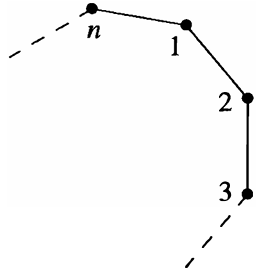
\includegraphics[width=0.25\textwidth]{images/fig1-1.png}
    \caption{}
    \label{fig1-1}
\end{figure}

于是，每个对称 \( s \) 都可以由 \(\{1, 2, 3, \dots, n\}\) 上相应的置换 \( \sigma \) 唯一描述，其中若对称 \( s \) 将顶点 \( i \) 放到顶点 \( j \) 原来的位置，则 \( \sigma \) 是将 \( i \) 映到 \( j \) 的置换。
例如，若 \( s \) 是绕 \( n \) 边形中心顺时针旋转 \( 2\pi/n \) 弧度，则 \( \sigma \) 是将 \( i \) 映到 \( i + 1 \)（\( 1 \leq i \leq n - 1 \)）且 \( \sigma(n) = 1 \) 的置换。
现在，通过对 \( s, t \in D_{2n} \) 定义 \( st \) 为先将 \( t \) 作用于 \( n \) 边形再作用 \( s \) 所得到的对称，将 \( D_{2n} \) 做成一个群（注意我们将对称视为 \( n \) 边形上的函数，因此 \( st \) 就是函数的复合——按通常的从右到左的读法）。
若 \( s, t \) 在顶点上分别实现置换 \( \sigma, \tau \)，则 \( st \) 实现 \( \sigma \circ \tau \). 
\( D_{2n} \) 上的二元运算是结合的，因为函数的复合是结合的。
\( D_{2n} \) 的单位元是恒等对称（保持所有顶点不动），记为 1，而 \( s \in D_{2n} \) 的逆元是逆转 \( s \) 的所有刚体运动的对称（因此若 \( s \) 在顶点上实现置换 \( \sigma \)，则 \( s^{-1} \) 实现 \( \sigma^{-1} \)）. 
在下一段中我们将证明
\[
|D_{2n}| = 2n,
\]
因此 \( D_{2n} \) 被称为 \( 2n \) 阶二面体群。
在某些教材中，这个群记为 \( D_n \)；然而，在群论文献中，\( D_{2n} \)（其中下标表示群的阶而不是顶点数）更为常见。

为了求阶 \(|D_{2n}|\)，注意到给定任意顶点 \(i\)，存在一个对称将顶点 1 送到位置 \(i\). 
由于顶点 2 与顶点 1 相邻，顶点 2 最终必在位置 \(i + 1\) 或 \(i - 1\)（其中 \(n + 1\) 视为 1，\(1 - 1\) 视为 \(n\)，即标号顶点的整数按模 \(n\) 读取）。
此外，在第一个对称之后，再对过顶点 \(i\) 和 \(n\) 边形中心的直线作反射，可以看出顶点 2 可以通过某个对称送到位置 \(i + 1\) 或 \(i - 1\) 中的任意一个。
因此，在对称作用下，有序顶点对 \((1, 2)\) 可以被送到 \(n \cdot 2\) 个位置。
%领域展开！
由于对称是刚体运动，一旦有序顶点对 \((1, 2)\) 的位置确定，对称在所有其余顶点上的作用就完全确定了。
因此，正 \(n\) 边形恰好有 \(2n\) 个对称。
此外，我们还可以明确地给出这 \(2n\) 个对称。
它们分别是绕中心旋转 \(2\pi i/n\) 弧度的 \(n\) 个旋转，\(0 \leq i \leq n - 1\)，以及关于 \(n\) 条对称轴的 \(n\) 个反射（若 \(n\) 为奇数，每条对称轴通过一个顶点和其对边的中点；若 \(n\) 为偶数，有 \(n/2\) 条对称轴通过两个相对顶点，另有 \(n/2\) 条对称轴垂直平分两条对边）。
例如，若 \(n = 4\)，在 \(x, y\) 平面中以原点画一个正方形，则对称轴为 \( x = 0 \)（\( y \) 轴）、\( y = 0 \)（\( x \) 轴）、\( y = x \) 和 \( y = -x \)（注意，通过原点的“反射”实际上不是反射，而是旋转 \( \pi \) 弧度）。

\begin{figure}[htbp]
    \centering
    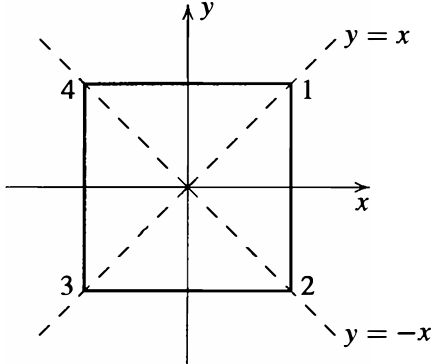
\includegraphics[width=0.4\textwidth]{images/fig1-2.png}
    \caption{}
    \label{fig1-2}
\end{figure}

由于二面体群将在全书中广泛用作例子，我们固定一些记号并提及一些计算，这些计算将简化未来的运算，并有助于将 \( D_{2n} \) 视为抽象群（而不必每次回到几何背景）。
在 \( x, y \) 平面中固定一个以原点为中心的正 \( n \) 边形，并沿顺时针方向将顶点依次标为 1 到 \( n \). 
设 \( r \) 为绕原点顺时针旋转 \( 2\pi / n \) 弧度的旋转。
设 \( s \) 为关于过顶点 1 和原点的对称轴的反射（我们对每个 \( n \) 使用相同的字母，但上下文总会明确 \( n \) 的值）。
我们将以下计算的细节留作练习（在大多数情况下我们将处理 \( D_6 \) 和 \( D_8 \)，因此读者可能希望先对 \( n = 3 \) 和 \( n = 4 \) 尝试这些练习）：

\begin{enumerate}[label=(\arabic*)]
\item\label{D_2n:(1)} \(1, r, r^2, \ldots, r^{n-1}\) 互不相同，且 \(r^n = 1\)，故 \(|r| = n\).
\item\label{D_2n:(2)} \(|s| = 2\).
\item\label{D_2n:(3)} 对任意 \(i\)，有\(s \neq r^i\) .
\item\label{D_2n:(4)} 对所有 \( 0 \leq i, j \leq n-1 \) 且 \( i \neq j \)，有 \( sr^i \neq sr^j \)，因此
\[
D_{2n} = \{1, r, r^2, \dots, r^{n-1}, s, sr, sr^2, \dots, sr^{n-1}\},
\]
即每个元素都可以唯一地写成 \( s^k r^i \) 的形式，其中 \( k = 0 \) 或 \( 1 \)，且 \( 0 \leq i \leq n-1 \).
\item \( rs = sr^{-1} \). [首先计算 \( s \) 在 \( \{1, 2, \dots, n\} \) 上实现什么置换，然后分别计算该等式两边对顶点 1 和 2 的作用.] 这特别表明 \( r \) 与 \( s \) 不可交换，因此 \( D_{2n} \) 是非阿贝尔的.
\item 对所有 \( 0 \leq i \leq n \)，\( r^i s = sr^{-i} \). [对 \( i \) 作归纳，并利用 \( r^{i+1} s = r(r^i s) \) 以及前面的计算结果.] 这说明了如何将 \( s \) 与 \( r \) 的幂交换。
\end{enumerate}


\subsection*{生成元与关系}

对二面体群使用生成元 \( r \) 和 \( s \) 提供了一种简明的方式在 \( D_{2n} \) 中进行计算。
我们可以类似地为任意群引入生成元和关系的概念。
尽早（在其形式化证明之前）掌握这些概念是有益的，因为它们为许多群提供了简单的描述和计算方法。
生成元将在 2.4 节中更详细地讨论，而这两个概念都将在 6.3 节引入自由群的概念时得到严格处理。

群 \( G \) 的元素的一个子集 \( S \)，若满足 \( G \) 中每个元素都可以写成 \( S \) 中元素及其逆元的（有限）乘积，则称 \( S \) 为 \( G \) 的一组\textbf{生成元}。
我们将在记号上写作 \( G = \langle S \rangle \)，并说 \( G \) 由 \( S \) \textbf{生成}，或 \( S \) \textbf{生成} \( G \)。
例如，整数 1 是整数加法群 \( \mathbb{Z} \) 的一个生成元，因为每个整数都是有限个 \(+1\) 与 \(-1\) 的和，所以 \( \mathbb{Z} = \langle 1 \rangle \). 
由 \( D_{2n} \) 的性质 \ref{D_2n:(4)}，集合 \( S = \{r, s\} \) 是 \( D_{2n} \) 的一组生成元，因此 \( D_{2n} = \langle r, s \rangle \)。我们后面将看到，在有限群 \( G \) 中，如果 \( G \) 的每个元素都是 \( S \) 中元素的有限乘积，则 \( S \) 生成 \( G \)（即不必再包含 \( S \) 中元素的逆元）。

一般群 \( G \) 中生成元满足的任何等式都称为 \( G \) 中的\textbf{关系}。
因此在 \( D_{2n} \) 中有关系：\( r^n = 1 \)，\( s^2 = 1 \) 以及 \( rs = sr^{-1} \)。
此外，在 \( D_{2n} \) 中，这三个关系还具有附加性质：群中元素之间的任何其他关系都可以从这三个关系导出（这并非显然；它出自以下事实：仅使用这三个关系就能确切判断两个群元素何时相等）。

一般地，若某个群 \( G \) 由子集 \( S \) 生成，并且存在一些关系，比如 \( R_1, R_2, \ldots, R_m \)（这里每个 \( R_i \) 是 \( S \cup \{1\} \) 中元素的方程），使得 \( S \) 中元素之间的任何关系都能从这些关系推出，则我们称这些生成元和关系为 \( G \) 的一个\textbf{表示}，并写作
\[
G = \langle S \mid R_1, R_2, \ldots, R_m \rangle.
\]

二面体群 \( D_{2n} \) 的一个表示（使用上述生成元和关系）为
\[
D_{2n} = \langle r, s \mid r^n = s^2 = 1,\ rs = sr^{-1} \rangle. \tag{1.1}
\]

我们将看到，使用这个表示来描述 \( D_{2n} \)（而不是总是回到原始的几何描述）将大大简化这些群的处理。

表示法提供了一种描述许多群的简单方法，但有一些微妙之处需要考虑。
其中之一是，在任意表示中，判断群的两个元素（用给定生成元表示）何时相等可能是困难的（甚至是不可能的）。
因此，所表示的群的阶是多少，甚至该群是有限还是无限，都可能不明显！
例如，可以证明 \( \langle x_1, y_1 \mid x_1^2 = y_1^2 = (x_1y_1)^2 = 1 \rangle \) 是一个 4 阶群的表示，而 \( \langle x_2, y_2 \mid x_2^3 = y_2^3 = (x_2y_2)^3 = 1 \rangle \) 是一个无限群的表示（见习题）。

另一个微妙之处是，即使在相当简单的表示中，也可能发生某种“坍缩”，因为关系以某种不明显的方式相互纠缠，即可能存在“隐藏的”或隐含的关系，它们没有在表示中明确给出，而是所给关系的推论。
这种坍缩使得通常甚至难以确定所表示的群的大小的下界。
例如，假设有人模仿 \( D_{2n} \) 的表示，试图通过定义另一个群：
\[
X_{2n} = \langle x, y \mid x^n = y^2 = 1,\ xy = yx^2 \rangle. \tag{1.2}
\]
“交换”关系 \( xy = yx^2 \) 决定了如何交换 \( y \) 和 \( x \)（即如何将 \( y \) 从 \( x \) 的右边“移到”左边），因此，正如在群 \( D_{2n} \) 中一样，这个群中的每个元素都可以写成 \( y^k x^i \) 的形式，其中所有 \( y \) 的幂在左边，所有\( x \) 的幂在右边。
此外，由前两个关系，\( x \) 和 \( y \) 的任何幂都可以化简，使得 \( i \) 介于 0 和 \( n-1 \) 之间，且 \( k \) 为 0 或 1.
因此人们可能认为 \( X_{2n} \) 再次是一个 \( 2n \) 阶群。
但事实并非如此，因为这个群中有一个由关系 \( x = xy^2 \)（因为 \( y^2 = 1 \)）通过反复应用交换关系和结合律将 \( y \) 移到左边而得到的“隐藏”关系：
\[
\begin{aligned}
x &= xy^2 = (xy)y = (yx^2)y = (yx)(xy) = (yx)(yx^2) \\
  &= y(xy)x^2 = y(yx^2)x^2 = y^2x^4 = x^4.
\end{aligned}
\]

由于 \( x^4 = x \)，由消去律得 \( X_{2n} \) 中 \( x^3 = 1 \)，并且由上面的讨论可知，对任意 \( n \)，\( X_{2n} \) 的阶至多为 6. 
根据 \( n \) 的值，还可能发生更多的坍缩（见习题）。

作为另一个例子，考虑表示
\[
Y = \langle u, v \mid u^4 = v^3 = 1,\ uv = v^2u^2 \rangle. \tag{1.3}
\]
在这种情况下，人们很容易猜测 \( Y \) 是一个 12 阶群，但同样存在额外的隐含关系。
事实上，这个群 \( Y \) 退化为 1 阶平凡群，即 \( u \) 和 \( v \) 满足额外关系 \( u = 1 \) 和 \( v = 1 \)（证明概述见习题）。

这种坍缩不会发生在 \( D_{2n} \) 的表示中，因为我们通过独立的（几何）方法证明存在一个 \( 2n \) 阶群，其生成元为 \( r \) 和 \( s \)，并且满足 \ref{D_2n:(1)} 中的关系。
因此，仅有这些关系的群的阶至少为 \( 2n \)。另一方面，容易看出（使用与上面 \( X_{2n} \) 类似的论证以及交换关系 \( rs = sr^{-1} \)）由 \ref{D_2n:(1)} 中的生成元和关系定义的任何群的阶至多为 \( 2n \)。因此，表示 \ref{D_2n:(1)} 所给出的群的阶恰好为 \( 2n \)，并且这个群确实就是正 \( n \) 边形的对称群。

我们对表示 \ref{D_2n:(1)} 所具有的额外信息是：存在一个已知阶的群满足这些信息。相比之下，我们对满足 \ref{D_2n:(2)} 或 \ref{D_2n:(3)} 中关系的任何群没有独立的认识。没有这种独立的“下界”信息，我们甚至可能无法确定一个给定的表示是否只是描述了平凡群，如 \ref{D_2n:(3)} 中的情况。

虽然一般来说，通过表示来规定群时必须非常小心，但对已知群使用表示法是一个强大的概念和计算工具。
关于表示的更多结果，包括更详细的例子，将在第 6.3 节中给出。

\subsection*{习题}
在以下习题中，\( D_{2n} \) 具有通常的表示 \( D_{2n} = \langle r, s \mid r^n = s^2 = 1,\ rs = sr^{-1} \rangle \).
\begin{enumerate}
\item 计算下列群中每个元素的阶：
\begin{enumerate}
\item \(D_6\)
\item \(D_8\)
\item \(D_{10}\).
\end{enumerate}
\item 利用生成元与关系证明：若 \(x \in D_{2n}\) 不是 \(r\) 的幂，则 \(rx = xr^{-1}\).
\item 证明 \(D_{2n}\) 中每个不是 \(r\) 的幂的元素都与 \(s\) 共轭，且阶为 2。
\item 若 \(n = 2k\) 是偶数且 \(n \ge 4\)，证明 \(z = r^k\) 是 2 阶元且与 \(D_{2n}\) 中所有元素可交换。证明 \(z\) 是唯一与所有元素可交换的非单位元。
\item 若 \(n\) 为奇数且 \(n \ge 3\)，证明单位元是 \(D_{2n}\) 中唯一与所有元素可交换的元素。
\item 设 \(x, y\) 是群 \(G\) 中的 2 阶元，令 \(t = xy\)。证明 \(tx = xt^{-1}\)。若 \(|xy| = n < \infty\)，则 \(x, t\) 满足与 \(D_{2n}\) 中 \(s, r\) 相同的关系。
\item 证明 \( \langle a, b \mid a^2 = b^2 = (ab)^n = 1 \rangle \) 给出了 \( D_{2n} \) 的一个用两个生成元 \( a = s \) 和 \( b = sr \)（它们在习题 3 中已计算出阶为 2）表示的表示。[证明 \( r \) 和 \( s \) 的关系可以从 \( a \) 和 \( b \) 的关系推出，反过来，\( a \) 和 \( b \) 的关系也可以从 \( r \) 和 \( s \) 的关系推出.]
\item 求 \(D_{2n}\) 中由 \(r\) 生成的循环子群的阶（参见第 1 节习题 27）。
\end{enumerate}

在习题 9 至 13 中，你可以通过遵循 \( D_{2n} \) 阶的证明来求出给定柏拉图立体在 \( \mathbb{R}^3 \) 中的刚体运动群（也称为旋转群）的阶：找出相邻顶点对可被送到的位置数。或者，你可以找出给定面可被送到的位置数，以及一旦一个面固定后，该面上一个顶点可被送到的位置数。
\begin{enumerate}[resume*]
\item 证明正四面体的空间刚体运动群阶为 12.
\item 证明立方体的空间刚体运动群阶为 24.
\item 证明正八面体的空间刚体运动群阶为 24.
\item 证明正十二面体的空间刚体运动群阶为 60.
\item 证明正二十面体的空间刚体运动群阶为 60.
\item 找出 \(\mathbb{Z}\) 的一组生成元。
\item 找出 \(\mathbb{Z}/n\mathbb{Z}\) 的一组生成元和关系。
\item 证明 \( \langle x_1, y_1 \mid x_1^2 = y_1^2 = (x_1y_1)^2 = 1 \rangle \) 是二面体群 \( D_4 \)（其中 \( x_1 \) 可用字母 \( r \) 代替，\( y_1 \) 用 \( s \) 代替）。[证明最后一个关系等价于 \( x_1y_1 = y_1x_1^{-1} \).]
\item 设 \( X_{2n} \) 是由 (1.2) 给出的群。
\begin{enumerate}[label=(\alph*)]
\item 证明若 \( n = 3k \)，则 \( X_{2n} \) 的阶为 6，且当 \( x \) 换为 \( r \)，\( y \) 换为 \( s \) 时，它具有与 \( D_6 \) 相同的生成元和关系。
\item 证明若 \( \gcd(3, n) = 1 \)，则 \( x \) 满足额外关系：\( x = 1 \). 在这种情况下，推出 \( X_{2n} \) 的阶为 2。[利用事实 \( x^n = 1 \) 和 \( x^3 = 1 \).]
\end{enumerate}
\item 设 \( Y \) 是由 (1.3) 给出的群。
\begin{enumerate}[label=(\alph*)]
\item 证明 \( v^2 = v^{-1} \).[利用关系 \( v^3 = 1 \).]
\item 证明 \( v \) 与 \( u^3 \) 可交换。[将左边写成 \( (v^2u^2)(uv) \) 并利用关系化简到右边，然后用 (a).]
\item 证明 \( v \) 与 \( u \) 可交换。[证明 \( u^9 = u \)，然后用 (b).]
\item 证明 \( uv = 1 \).[用 (c) 和最后一个关系。]
\item 证明 \( u = 1 \)，推出 \( v = 1 \)，并由此得出 \( Y = 1 \).[用 (d) 和方程 \( u^4v^3 = 1 \).]
\end{enumerate}
\end{enumerate}


\section{对称群}

设 \(\Omega\) 为任意非空集合，并令 \(S_\Omega\) 为从 \(\Omega\) 到自身的所有双射的集合（即 \(\Omega\) 的所有置换的集合）。
集合 \(S_\Omega\) 在函数复合 \(\circ\) 下构成群。
注意 \(\circ\) 是 \(S_\Omega\) 上的二元运算，因为若 \(\sigma : \Omega \to \Omega\) 和 \(\tau : \Omega \to \Omega\) 都是双射，则 \(\sigma \circ \tau\) 也是从 \(\Omega\) 到 \(\Omega\) 的双射。
由于函数复合一般是结合的，\(\circ\) 是结合的。
\(S_\Omega\) 的单位元是由“对所有 \(a \in \Omega\)，\(1(a) = a\)”定义的置换 1。
对每个置换 \(\sigma\)，存在一个（双边）逆函数 \(\sigma^{-1} : \Omega \to \Omega\)，满足 \(\sigma \circ \sigma^{-1} = \sigma^{-1} \circ \sigma = 1\). 
因此，\((S_\Omega, \circ)\) 满足所有群公理。
这个群称为集合 \(\Omega\) 上的\textbf{对称群}。
重要的是要认识到，\(S_\Omega\) 的元素是 \(\Omega\) 的\textbf{置换}，而不是 \(\Omega\) 本身的元素。

在特殊情形 \(\Omega = \{1, 2, 3, \ldots, n\}\) 时，\(\Omega\) 上的对称群记为 \(S_n\)，称为 \(n\) 次\textbf{对称群}。
群 \(S_n\) 将在全文中扮演重要角色，既作为自身具有相当研究兴趣的群，也作为说明和推动一般理论的手段。

首先我们证明 \(S_n\) 的阶为 \(n!\). 
\(\{1, 2, 3, \ldots, n\}\) 的置换正是该集合到自身的单射函数，因为它是有限的（命题 \ref{pro:0-1}），并且我们可以计算单射函数的个数。
一个单射函数 \(\sigma\) 可以将数字 1 送到 \(\{1, 2, 3, \ldots, n\}\) 中的任意 \(n\) 个元素之一；\(\sigma(2)\) 则可以是该集合中除 \(\sigma(1)\) 外的任意元素（因此 \(\sigma(2)\) 有 \(n-1\) 种选择）；\(\sigma(3)\) 可以是除 \(\sigma(1)\) 或 \(\sigma(2)\) 外的任意元素（因此 \(\sigma(3)\) 有 \(n-2\) 种选择），依此类推。
因此，从 \(\{1, 2, 3, \ldots, n\}\) 到自身的单射函数共有 \(n \cdot (n-1) \cdot (n-2) \cdots 2 \cdot 1 = n!\) 个。
因此 \(\{1, 2, 3, \ldots, n\}\) 恰好有 \(n!\) 个置换，所以 \(S_n\) 中恰好有 \(n!\) 个元素。

我们现在描述一种高效的记号来书写 \( S_n \) 的元素 \( \sigma \)，这个记号将在全文中使用，称为\textbf{轮换分解}。

一个\textbf{轮换}是一个整数串，它表示 \( S_n \) 中循环置换这些整数（并固定所有其他整数）的元素。
轮换 \( (a_1 \, a_2 \, \dots \, a_m) \) 是将 \( a_i \) 送到 \( a_{i+1} \)（\( 1 \leq i \leq m-1 \)）并将 \( a_m \) 送到 \( a_1 \) 的置换。
例如，\( (2 \, 1 \, 3) \) 是将 2 映到 1、1 映到 3、3 映到 2 的置换。
一般地，对每个 \( \sigma \in S_n \)，数字 1 到 \( n \) 将被重新排列并分成 \( k \) 个轮换，形式为
\[
(a_1 \, a_2 \, \dots \, a_{m_1})(a_{m_1+1} \, a_{m_1+2} \, \dots \, a_{m_2}) \cdots (a_{m_{k-1}+1} \, a_{m_{k-1}+2} \, \dots \, a_{m_k}),
\]
从中可以容易地读出 \( \sigma \) 在 1 到 \( n \) 中任意数上的作用，如下所述。
对任意 \( x \in \{1, 2, 3, \dots, n\} \)，首先在上述表达式中定位 \( x \). 
如果 \( x \) 后面不紧跟右括号（即 \( x \) 不在 \( k \) 个轮换中某一个的右端），则 \( \sigma(x) \) 是紧接在 \( x \) 右边的整数。
如果 \( x \) 后面跟着右括号，则 \( \sigma(x) \) 是以 \( x \) 结尾的那个轮换开头的数字（即，若 \( x = a_{m_i} \)（对某个 \( i \)），则 \( \sigma(x) = a_{m_{i-1}+1} \)（其中 \( m_0 \) 取为 0））。
我们可以将这个对 \( \sigma \) 的描述表示如图：

\begin{figure}[htbp]
    \centering
    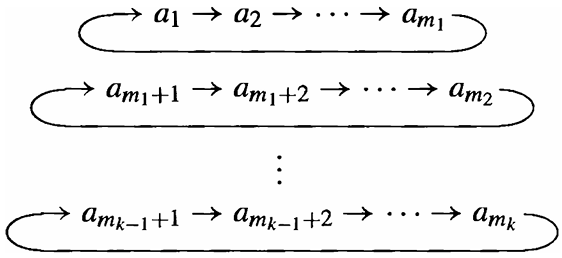
\includegraphics[width=0.6\textwidth]{images/fig1-3.png}
    \caption{}
    \label{fig1-3}
\end{figure}

所有轮换的乘积称为 \( \sigma \) 的\textbf{轮换分解}。

我们现在给出计算 \( S_n \) 中元素 \( \sigma \) 的轮换分解的算法，并用一个具体的置换逐步演示该算法。
我们将这个算法的证明以及轮换分解唯一性方面的完整分析推迟到第 4 章。


设 \( n = 13 \)，并令 \( \sigma \in S_{13} \) 定义为
\[
\begin{aligned}
\sigma(1) = 12, 
\quad \sigma(2) = 13, 
\quad \sigma(3) = 3, 
\quad \sigma(4) = 1, 
\quad \sigma(5) = 11, \\
\sigma(6) = 9, 
\quad \sigma(7) = 5, 
\quad \sigma(8) = 10, 
\quad \sigma(9) = 6, 
\quad \sigma(10) = 4,
\\
\sigma(11) = 7, 
\quad \sigma(12) = 8, 
\quad \sigma(13) = 2.
\end{aligned}
\]

\begin{tabular}{|p{9cm}|p{4cm}|}
\hline
\textbf{方法} & \textbf{示例} \\
\hline
开始一个新轮换：选取 \(\{1, 2, \dots, n\}\) 中尚未出现在之前轮换里的最小元素，记为 \(a\)（若刚开始，则 \(a = 1\)）；开始新轮换：\((a\) & \((1\) \\
\hline
从给定的 \(\sigma\) 描述中读出 \(\sigma(a)\)，记为 \(b\). 
若 \(b = a\)，用右括号关闭该轮换（不写出 \(b\)）；此轮换完成，返回第 1 步。
若 \(b \neq a\)，在本轮换中把 \(b\) 写在 \(a\) 旁边：\((a\,b\) & \(\sigma(1) = 12 = b\)，且 \(12 \neq 1\)，因此写出：\((1\,12\) \\
\hline
从给定的 \(\sigma\) 描述中读出 \(\sigma(b)\)，记为 \(c\). 
若 \(c = a\)，用右括号关闭该轮换；返回第 1 步。
若 \(c \neq a\)，在本轮换中把 \(c\) 写在 \(b\) 旁边：\((a\,b\,c\). 
重复此步骤，将 \(c\) 作为新的 \(b\) 值，直到轮换闭合为止。 
& \(\sigma(12) = 8\)，且 \(8 \neq 1\)，因此继续轮换为：\((1\,12\,8\) \\
\hline
\end{tabular}
\vspace{\baselineskip}

自然地，当 \(\{1, 2, \dots, n\}\) 中的所有数都已出现在某个轮换中时，这个过程就停止了。
对于例子中的特定 \(\sigma\)，这给出
\[
\sigma = (1\ 12\ 8\ 10\ 4)(2\ 13)(3)(5\ 11\ 7)(6\ 9).
\]

一个轮换的\textbf{长度}是出现在其中的整数的个数。
长度为 \(t\) 的轮换称为 \textbf{\(t\)-轮换}。
两个轮换若没有公共的数字，则称为\textbf{不相交}的。
因此，上面的元素 \(\sigma\) 是 5 个（两两）不相交轮换的乘积：一个 5-轮换、一个 2-轮换、一个 1-轮换、一个 3-轮换，以及另一个 2-轮换。

从现在起，我们采用省略 1-轮换的约定。
因此，若某个整数 \(i\) 没有出现在置换 \(\tau\) 的轮换分解中，则理解为 \(\tau(i) = i\)，即 \(\tau\) 固定 \(i\). 
\(S_n\) 的恒等置换的轮换分解为 \((1)(2)\cdots(n)\)，将简写为 1。
于是算法的最后一步为：

\begin{tabular}{|p{9cm}|p{4cm}|}
\hline
最终步骤：删除所有长度为 1 的轮换
\hline
\end{tabular}
\vspace{\baselineskip}

因此，例子中特定 \(\sigma\) 的轮换分解为
\[
\sigma = (1\ 12\ 8\ 10\ 4)(2\ 13)(5\ 11\ 7)(6\ 9).
\]
这个约定的好处是：\(S_n\) 中元素 \(\tau\) 的轮换分解，同时也是 \(S_m\)（\(m \geq n\)）中那个在 \(\{1, 2, 3, \dots, n\}\) 上作用与 \(\tau\) 相同、并固定 \(\{n+1, n+2, \dots, m\}\) 中每个元素的置换的轮换分解。
因此，例如，\((1\ 2)\) 是互换 1 和 2 并固定所有更大的整数的置换，无论在 \(S_2\), \(S_3\) 还是 \(S_4\) 等中看待都是如此。

作为另一个例子，\(S_3\) 的 6 个元素具有如下的轮换分解：

\begin{table}[h!]
    \centering
    \caption{群 \( S_3 \)}
    \begin{tabular}{|c|c|}
\hline
\( \sigma_i \) 的取值 & \( \sigma_i \) 的轮换分解 \\
\hline
\(\sigma_1(1) = 1,\ \sigma_1(2) = 2,\ \sigma_1(3) = 3\) & 1 \\
\(\sigma_2(1) = 1,\ \sigma_2(2) = 3,\ \sigma_2(3) = 2\) & (2 3) \\
\(\sigma_3(1) = 3,\ \sigma_3(2) = 2,\ \sigma_3(3) = 1\) & (1 3) \\
\(\sigma_4(1) = 2,\ \sigma_4(2) = 1,\ \sigma_4(3) = 3\) & (1 2) \\
\(\sigma_5(1) = 2,\ \sigma_5(2) = 3,\ \sigma_5(3) = 1\) & (1 2 3) \\
\hline
\end{tabular}
    \label{tab:placeholder}
\end{table}

对任意 \( \sigma \in S_n \)，\( \sigma^{-1} \) 的轮换分解可通过将 \( \sigma \) 的轮换分解中每个轮换里的数字按相反顺序写出而得到。
例如，若
$\sigma = (1\ 12\ 8\ 10\ 4)(2\ 13)(5\ 11\ 7)(6\ 9) $
是前面描述的 \( S_{13} \) 中的元素，则
\[ \sigma^{-1} = (4\ 10\ 8\ 12\ 1)(13\ 2)(7\ 11\ 5)(9\ 6). \]

在 \( S_n \) 中计算乘积是直接的，只要记住在计算 \( \sigma \circ \tau \) 时，要从右向左读置换。
只需“跟随”元素在相继置换下的像即可。
例如，在乘积 (1 2 3) \(\circ\) (1 2)(3 4) 中，数字 1 被第一个置换送到 2，然后 2 被第二个置换送到 3，因此复合映射将 1 送到 3。
要计算该乘积的轮换分解，接下来需要看 3 的情况。
它先被送到 4，然后 4 被固定，所以复合映射将 3 送到 4。
类似地，4 先被送到 3，然后 3 被送到 1，从而完成乘积中的这个轮换：\((1 \, 3 \, 4)\). 
最后，2 被送到 1，然后 1 被送到 2，因此 2 被该乘积固定，所以 \((1 \, 2 \, 3) \circ (1 \, 2)(3 \, 4) = (1 \, 3 \, 4)\) 就是该乘积的轮换分解。

作为更多的例子，
\[
(12) \circ (13) = (1 \, 3 \, 2) \quad \text{与} \quad (1 \, 3) \circ (1 \, 2) = (1 \, 2 \, 3).
\]
特别地，这表明
\[
S_n \text{ 对所有 } n \geq 3 \textbf{ 都是非阿贝尔群}.
\]

轮换分解中的每个轮换 \((a_1 \, a_2 \, \ldots \, a_m)\) 都可看作循环置换 \(a_1, a_2, \ldots, a_m\) 并固定所有其他整数的置换。
由于不相交的轮换置换的是不相交集合中的数字，因此有
\[
\textbf{不相交的轮换可交换}.
\]
因此，在任何不相交轮换的乘积（特别是轮换分解）中重新排列轮换的顺序不会改变置换。

此外，由于给定轮换 \((a_1 \, a_2 \, \ldots \, a_m)\) 循环地置换 \(\{a_1, a_2, \ldots, a_m\}\)，轮换中的数字可以循环地重排而不改变置换，即
\[
(a_1 \, a_2 \, \ldots \, a_m) = (a_2 \, a_3 \, \ldots \, a_m \, a_1) = (a_3 \, a_4 \, \ldots \, a_m \, a_1 \, a_2) = \cdots = (a_m \, a_1 \, a_2 \, \ldots \, a_{m-1}).
\]
因此，例如，\((1 \, 2) = (2 \, 1)\) 且 \((1 \, 2 \, 3 \, 4) = (3 \, 4 \, 1 \, 2)\). 
按惯例，轮换中出现的最小数通常写在最前面。

使用轮换时必须小心，因为一个置换可以以多种方式写成轮换的任意乘积。
例如，在 \(S_3\) 中，
\((1 \, 2 \, 3) = (1 \, 2)(2 \, 3) = (1 \, 3)(1 \, 3 \, 2)(1 \, 3)\) 等等。
但（如我们将要证明的）每个置换的轮换分解是将置换表示为不相交轮换的乘积的唯一方式（除了重新排列轮换和轮换内数字的循环重排外）。
将轮换的任意乘积化为不相交轮换的乘积，使我们能一眼判定两个置换是否相同。
这种记号的另一个优点是，证明\textbf{置换的阶等于其轮换分解中各轮换长度的最小公倍数}是一个习题（下面概述）。



\subsection*{习题}

\begin{enumerate}
\item 设 \( \sigma \) 为置换
\[
1 \mapsto 3 \quad 2 \mapsto 4 \quad 3 \mapsto 5 \quad 4 \mapsto 2 \quad 5 \mapsto 1,
\]
且 \( \tau \) 为置换
\[
1 \mapsto 5 \quad 2 \mapsto 3 \quad 3 \mapsto 2 \quad 4 \mapsto 4 \quad 5 \mapsto 1.
\]
求下列每个置换的轮换分解：\( \sigma, \tau, \sigma^2, \sigma\tau, \tau\sigma \) 及 \( \tau^2\sigma \).

\item 设 \( \sigma \) 为置换
\[
\begin{aligned}
1 \mapsto 13,&\quad 2 \mapsto 2,\quad 3 \mapsto 15,\quad 4 \mapsto 14,\quad 5 \mapsto 10,\\
6 \mapsto 6,&\quad 7 \mapsto 12,\quad 8 \mapsto 3,\quad 9 \mapsto 4,\quad 10 \mapsto 1,\\
11 \mapsto 7,&\quad 12 \mapsto 9,\quad 13 \mapsto 5,\quad 14 \mapsto 11,\quad 15 \mapsto 8,
\end{aligned}
\]
且 \( \tau \) 为置换
\[
\begin{aligned}
1 \mapsto 14,&\quad 2 \mapsto 9,\quad 3 \mapsto 10,\quad 4 \mapsto 2,\quad 5 \mapsto 12,\\
6 \mapsto 6,&\quad 7 \mapsto 5,\quad 8 \mapsto 11,\quad 9 \mapsto 15,\quad 10 \mapsto 3,\\
11 \mapsto 8,&\quad 12 \mapsto 7,\quad 13 \mapsto 4,\quad 14 \mapsto 1,\quad 15 \mapsto 13.
\end{aligned}
\]
求下列置换的轮换分解：\( \sigma, \tau, \sigma^2, \sigma\tau, \tau\sigma \) 及 \( \tau^2\sigma \).

\item 对前两题中已求出轮换分解的每个置换，计算其阶.

\item 计算下列群中每个元素的阶：
\begin{enumerate}[label=(\alph*)]
\item \( S_3 \);
\item \( S_4 \).
\end{enumerate}

\item 求 \( (1 \ 12 \ 8 \ 10 \ 4)(2 \ 13)(5 \ 11 \ 7)(6 \ 9) \) 的阶.

\item 写出 \( S_4 \) 中每个 4 阶元的轮换分解.

\item 写出 \( S_4 \) 中每个 2 阶元的轮换分解.

\item 证明若 \( \Omega = \{1, 2, 3, \dots\} \)，则 \( S_\Omega \) 是无限群（不要说 \( \infty! = \infty \)）.

\item \begin{enumerate}[label=(\alph*)]
\item 设 \( \sigma \) 为 12-轮换 \( (1 \ 2 \ 3 \ 4 \ 5 \ 6 \ 7 \ 8 \ 9 \ 10 \ 11 \ 12) \). 对哪些正整数 \( i \)，\( \sigma^i \) 也是 12-轮换？
\item 设 \( \tau \) 为 8-轮换 \( (1 \ 2 \ 3 \ 4 \ 5 \ 6 \ 7 \ 8) \). 对哪些正整数 \( i \)，\( \tau^i \) 也是 8-轮换？
\item 设 \( \omega \) 为 14-轮换 \( (1 \ 2 \ 3 \ 4 \ 5 \ 6 \ 7 \ 8 \ 9 \ 10 \ 11 \ 12 \ 13 \ 14) \). 对哪些正整数 \( i \)，\( \omega^i \) 也是 14-轮换？
\end{enumerate}

\item 证明若 \( \sigma \) 是 \( m \)-轮换 \( (a_1 \ a_2 \ \dots \ a_m) \)，则对所有 \( i \in \{1, 2, \dots, m\} \)，\( \sigma^i(a_k) = a_{k+i} \)，其中当 \( k+i > m \) 时 \( k+i \) 用其模 \( m \) 的最小剩余代替。由此推出 \( |\sigma| = m \).

\item 设 \( \sigma \) 为 \( m \)-轮换 \( (1 \ 2 \ \dots \ m) \). 证明 \( \sigma^i \) 也是 \( m \)-轮换当且仅当 \( i \) 与 \( m \) 互素.

\item \begin{enumerate}[label=(\alph*)]
\item 若 \( \tau = (1 \ 2)(3 \ 4)(5 \ 6)(7 \ 8)(9 \ 10) \)，判断是否存在一个 \( n \)-轮换 \( \sigma \)（\( n \geq 10 \)）使得对某个整数 \( k \) 有 \( \tau = \sigma^k \).
\item 若 \( \tau = (1 \ 2)(3 \ 4 \ 5) \)，判断是否存在一个 \( n \)-轮换 \( \sigma \)（\( n \geq 5 \)）使得对某个整数 \( k \) 有 \( \tau = \sigma^k \).
\end{enumerate}

\item 证明 \( S_n \) 中一个元素的阶为 2 当且仅当其轮换分解是一组两两不相交的对换的乘积.

\item 设 \( p \) 为素数。证明 \( S_n \) 中一个元素的阶为 \( p \) 当且仅当其轮换分解是一组两两不相交的 \( p \)-轮换的乘积。通过一个具体例子说明，若 \( p \) 不是素数，则结论不一定成立.

\item 证明 \( S_n \) 中元素的阶等于其轮换分解中各轮换长度的最小公倍数。[利用习题 10 和第 1 节习题 24.]

\item 证明若 \( n \geq m \)，则 \( S_n \) 中 \( m \)-轮换的个数为
\[
\frac{n(n-1)(n-2)\cdots(n-m+1)}{m}.
\]
[计算构成一个 \( m \)-轮换的方式数，再除以一个特定 \( m \)-轮换的表示个数.]

\item 证明若 \( n \geq 4 \)，则 \( S_n \) 中可写成两个不相交 2-轮换之积的置换的个数为
\[
\frac{n(n-1)(n-2)(n-3)}{8}.
\]

\item 找出所有整数 \( n \)，使得 \( S_5 \) 中含有 \( n \) 阶元。[利用习题 15.]

\item 找出所有整数 \( n \)，使得 \( S_7 \) 中含有 \( n \) 阶元。[利用习题 15.]

\item 找出 \( S_3 \) 的一组生成元和关系。

\end{enumerate}

\section{矩阵群}

在本节中，我们引入系数来自域的矩阵群的概念。这个群族例子将在第一部分中用于说明目的，并在向量空间的章节中进行更详细的研究。

域是能够进行所有算术运算 \( + \), \( - \), \( \times \) 和 \( \div \)（除以非零元）的“最小”数学结构，因此特别地，每个非零元都必须有乘法逆元。
我们将在后面更深入地研究域，在本部分的文本中，我们将遇到的域只有 \( \mathbb{Q} \), \( \mathbb{R} \) 和 \( \mathbb{Z}/p\mathbb{Z} \)（其中 \( p \) 是素数）。
例子 \( \mathbb{Z}/p\mathbb{Z} \) 是一个有限域，为了强调它是个域，我们将它记为 \( \mathbb{F}_p \). 
为完整起见，我们在此给出域的精确定义。

\begin{definition}
\begin{enumerate}
\item 一个\textbf{域}是一个集合 \( F \)，连同 \( F \) 上的两个二元运算 \(+\) 和 \(\cdot\)，使得 \((F, +)\) 是阿贝尔群（称其单位元为 0），\((F - \{0\}, \cdot)\) 也是阿贝尔群，并且满足以下\textbf{分配律}：
\[
a \cdot (b + c) = (a \cdot b) + (a \cdot c), \quad \text{对所有 } a, b, c \in F.
\]
\item 对任意域 \( F \)，记 \( F^\times = F - \{0\} \).
\end{enumerate}
\end{definition}

所有标量来自 \(\mathbb{R}\) 时的向量空间理论、矩阵与线性变换理论以及行列式理论，在标量来自任意域 \( F \) 时（\textbf{作适当修改后}）仍然成立。
当我们在第一部分使用这些理论时，会明确说明我们所假设的关于域的事实。

对每个 \( n \in \mathbb{Z}^+ \)，令 \( GL_n(F) \) 为所有元素来自 \( F \) 且行列式非零的 \( n \times n \) 矩阵的集合，即
\[
GL_n(F) = \{A \mid A \text{ 是元素来自 } F \text{ 的 } n \times n \text{ 矩阵，且 } \det(A) \neq 0\},
\]
其中元素来自 \( F \) 的任意矩阵 \( A \) 的行列式可用与 \( F = \mathbb{R} \) 时相同的公式计算。
对任意 \( n \times n \) 矩阵 \( A \) 和 \( B \)，令 \( AB \) 为按与 \( F = \mathbb{R} \) 时相同的规则计算出的乘积。
这个乘积是结合的。
此外，由于 \( \det(AB) = \det(A) \cdot \det(B) \)，若 \( \det(A) \neq 0 \) 且 \( \det(B) \neq 0 \)，则 \( \det(AB) \neq 0 \)，所以 \( GL_n(F) \) 在矩阵乘法下封闭。
进一步地，\( \det(A) \neq 0 \) 当且仅当 \( A \) 有矩阵逆（且该逆可用与 \( F = \mathbb{R} \) 时相同的伴随公式计算），因此每个 \( A \in GL_n(F) \) 在 \( GL_n(F) \) 中都有逆元 \( A^{-1} \)：
\[
AA^{-1} = A^{-1}A = I,
\]
其中 \( I \) 是 \( n \times n \) 单位矩阵。
因此 \( GL_n(F) \) 在矩阵乘法下构成群，称为 \textbf{\( n \) 次一般线性群}。

以下结果将在第三部分中证明，但现在为了方便起见予以记录：
\begin{enumerate}[label=\arabic*]
\item 若 \( F \) 是域且 \( |F| < \infty \)，则对某个素数 \( p \) 和整数 \( m \)，有 \( |F| = p^m \)；
\item 若 \( |F| = q < \infty \)，则
\[
|GL_n(F)| = (q^n - 1)(q^n - q)(q^n - q^2)\cdots(q^n - q^{n-1}).
\]
\end{enumerate}

\subsection*{习题}

\begin{enumerate}
\item 证明 \( |GL_2(\mathbb{F}_2)| = 6 \).

\item 写出 \( GL_2(\mathbb{F}_2) \) 的所有元素，并计算每个元素的阶。

\item 证明 \( GL_2(\mathbb{F}_2) \) 是非阿贝尔的。

\item 证明若 \( n \) 不是素数，则 \( \mathbb{Z}/n\mathbb{Z} \) 不是域。

\item 证明 \( GL_n(F) \) 是有限群当且仅当 \( F \) 只有有限多个元素。

\item 若 \( |F| = q \) 有限，证明 \( |GL_n(F)| < q^{n^2} \)。

\item 设 \( p \) 为素数。证明 \( GL_2(\mathbb{F}_p) \) 的阶为 \( p^4 - p^3 - p^2 + p \)（不要直接引用本节中的阶公式）。[从 \( \mathbb{F}_p \) 上 \( 2 \times 2 \) 矩阵的总数中减去不可逆矩阵的个数。你可使用事实：一个 \( 2 \times 2 \) 矩阵不可逆当且仅当某一行是另一行的倍数。]

\item 证明对任意 \( n \geq 2 \) 和任意域 \( F \)，\( GL_n(F) \) 是非阿贝尔的。

\item 证明实 \( 2 \times 2 \) 矩阵的乘法运算作为二元运算是结合的。

\item 设
\[
G = \left\{ \begin{pmatrix} a & b \\ 0 & c \end{pmatrix} \,\middle|\, a, b, c \in \mathbb{R},\ a \neq 0,\ c \neq 0 \right\}.
\]
\begin{enumerate}[label=(\alph*)]
\item 计算 \( \begin{pmatrix} a_1 & b_1 \\ 0 & c_1 \end{pmatrix} \) 与 \( \begin{pmatrix} a_2 & b_2 \\ 0 & c_2 \end{pmatrix} \) 的乘积，以证明 \( G \) 在矩阵乘法下封闭。
\item 求 \( \begin{pmatrix} a & b \\ 0 & c \end{pmatrix} \) 的矩阵逆，并推出 \( G \) 在取逆下封闭。
\item 推出 \( G \) 是 \( GL_2(\mathbb{R}) \) 的一个子群（见第 1 节习题 26）。
\item 证明 \( G \) 中两个对角元相等（即 \( a = c \)）的元素组成的集合也是 \( GL_2(\mathbb{R}) \) 的一个子群。
\end{enumerate}

\item 下面的习题引入域 \( F \) 上的\textbf{海森堡群}，并发展其一些基本性质。当 \( F = \mathbb{R} \) 时，该群通过给出海森堡不确定性原理的群论解释（归功于 H. Weyl），在量子力学和信号理论中扮演重要角色。注意，海森堡群也可以更一般地定义——例如，元素来自 \( \mathbb{Z} \).

设
\[
H(F) = \left\{ \begin{pmatrix} 1 & a & b \\ 0 & 1 & c \\ 0 & 0 & 1 \end{pmatrix} \,\middle|\, a, b, c \in F \right\}
\]
称为 \( F \) 上的\textbf{海森堡群}。令
\[
X = \begin{pmatrix} 1 & a & b \\ 0 & 1 & c \\ 0 & 0 & 1 \end{pmatrix}, \qquad
Y = \begin{pmatrix} 1 & d & e \\ 0 & 1 & f \\ 0 & 0 & 1 \end{pmatrix}
\]
为 \( H(F) \) 中的元素。
\begin{enumerate}[label=(\alph*)]
\item 计算矩阵乘积 \( XY \)，并推出 \( H(F) \) 在矩阵乘法下封闭。
给出具体矩阵例子使得 \( XY \neq YX \)（从而 \( H(F) \) 总是非阿贝尔的）。
\item 给出矩阵逆 \( X^{-1} \) 的显式公式，并由此推出 \( H(F) \) 对逆封闭.
\item 证明 \( H(F) \) 的结合律，并推出 \( H(F) \) 是一个阶为 \( |F|^3 \) 的群。（不要假定矩阵乘法是结合的。）
\item 求有限群 \( H(\mathbb{Z}/2\mathbb{Z}) \) 中每个元素的阶。
\item 证明 \( H(\mathbb{R}) \) 中每个非单位元都有无限阶。
\end{enumerate}
\end{enumerate}

\section{四元数群}

\textbf{四元数群} \(Q_8\) 定义为
\[
Q_8 = \{1, -1, i, -i, j, -j, k, -k\},
\]
其乘法 \(\cdot\) 按以下规则计算：
\[
1 \cdot a = a \cdot 1 = a, \quad \text{对所有 } a \in Q_8,
\]
\[
(-1) \cdot (-1) = 1, \quad (-1) \cdot a = a \cdot (-1) = -a, \quad \text{对所有 } a \in Q_8,
\]
\[
i \cdot i = j \cdot j = k \cdot k = -1,
\]
\[
i \cdot j = k, \quad j \cdot i = -k,
\]
\[
j \cdot k = i, \quad k \cdot j = -i,
\]
\[
k \cdot i = j, \quad i \cdot k = -j.
\]

今后我们将 \( a \cdot b \) 简写为 \( ab \). 
验证结合律是繁琐的（我们稍后将用不那么计算性的方法证明），但其他公理很容易验证。
注意 \( Q_8 \) 是一个 8 阶非阿贝尔群。

\subsection*{习题}

\begin{enumerate}
\item 计算 \(Q_8\) 中每个元素的阶。
\item 写出 \(S_3, D_8, Q_8\) 的群表。
\item 找出 \(Q_8\) 的一组生成元和关系。
\end{enumerate}

\section{同态与同构}

在本节中，我们精确地给出两个群何时“看起来相同”的概念，即它们具有完全相同的群论结构。
这就是两个群之间的\textbf{同构}的概念。
我们首先定义\textbf{同态}的概念，关于这个概念我们将在后面有更多的论述。

\begin{definition}
设 \((G, \star)\) 和 \((H, \diamond)\) 是群。
一个映射 \(\varphi : G \to H\)，若满足
\[
\varphi(x \star y) = \varphi(x) \diamond \varphi(y), \quad \text{对所有 } x, y \in G,
\]
则称为\textbf{同态}。
\end{definition}

当 \( G \) 和 \( H \) 的群运算没有明确写出时，同态条件简化为
\[
\varphi(xy) = \varphi(x)\varphi(y),
\]
但重要的是要记住，左边的乘积 \( xy \) 是在 \( G \) 中计算的，而右边的乘积 \( \varphi(x)\varphi(y) \) 是在 \( H \) 中计算的。
直观地说，一个映射 \( \varphi \) 若保持其定义域和陪域的群结构，则称为同态。

\begin{definition}
映射 \( \varphi : G \to H \) 称为\textbf{同构}，并称 \( G \) 与 \( H \) \textbf{同构}或具有相同的\textbf{同构类型}，记为 \( G \cong H \)，如果
\begin{enumerate}[label=(\arabic*)]
\item \( \varphi \) 是同态（即 \( \varphi(xy) = \varphi(x)\varphi(y) \)），且
\item \( \varphi \) 是双射。
\end{enumerate}
换言之，若 \( G \) 与 \( H \) 之间存在一个保持群运算的双射，则它们同构。
直观地，\( G \) 与 \( H \) 是同一个群，只是元素和运算在 \( G \) 和 \( H \) 中可能写法不同。
因此，\( G \) 所具有的任何仅依赖于 \( G \) 的群结构的性质（即可以从群公理推导出来的性质，例如群的交换性）在 \( H \) 中也成立。
注意，这正式证明了将我们所有的群运算写作 \(\cdot\) 是合理的，因为改变运算的符号不会改变同构类型。
\end{definition}

\begin{example}
\begin{enumerate}[label=(\arabic*)]
\item 对任意群 \( G \)，有 \( G \cong G \). 
恒等映射给出一个显然的同构，但一般不是从 \( G \) 到自身的\textbf{唯一}同构。
更一般地，设 \( \mathcal{G} \) 是任意非空群族。
容易验证关系 \( \cong \) 是 \( \mathcal{G} \) 上的等价关系，其等价类称为\textbf{同构类}。
这解释了“同构”定义中有些对称性的措辞。

\item 指数映射 \( \exp : \mathbb{R} \to \mathbb{R}^+ \)，定义为 \( \exp(x) = e^x \)，其中 \( e \) 是自然对数的底，是从 \( (\mathbb{R}, +) \) 到 \( (\mathbb{R}^+, \times) \) 的同构。
\( \exp \) 是双射，因为它有反函数（即 \( \log_e \)），并且 \( \exp \) 保持群运算，因为 \( e^{x+y} = e^x e^y \). 
在这个例子中，元素和运算都不同，但两个群同构，即作为群它们具有相同的结构。

\item 在这个例子中，我们证明对称群的同构类型只取决于被置换的底集的基数。

设 \( \Delta \) 和 \( \Omega \) 是非空集合。
若 \( |\Delta| = |\Omega| \)，则对称群 \( S_\Delta \) 与 \( S_\Omega \) 同构。
我们可以直观地理解如下：给定 \( |\Delta| = |\Omega| \)，存在一个从 \( \Delta \) 到 \( \Omega \) 的双射 \( \theta \).
把 \( \Delta \) 和 \( \Omega \) 的元素通过 \( \theta \) “粘合”在一起，即每个 \( x \in \Delta \) 粘合到 \( \theta(x) \in \Omega \). 
要得到一个映射 \( \varphi : S_\Delta \to S_\Omega \)，设 \( \sigma \in S_\Delta \) 是 \( \Delta \) 的一个置换，并令 \( \varphi(\sigma) \) 为 \( \Omega \) 的置换，
%又用神之一令放大招了
它以 \( \sigma \) 移动 \( \Delta \) 中对应粘合元素的相同方式移动 \( \Omega \) 的元素；即，若对某些 \( x, y \in \Delta \) 有 \( \sigma(x) = y \)，则 \( \varphi(\sigma)(\theta(x)) = \theta(y) \) 在 \( \Omega \) 中成立。
由于集合双射 \( \theta \) 有逆，容易验证对称群之间的映射也有逆。
映射 \( \varphi \) 的精确技术定义以及确保 \( \varphi \) 是同构的那些性质的直接但繁琐的验证，留待下面的习题中完成。
%你把最好吃的一块吃给我看是吧

反过来，若 \( S_\Delta \cong S_\Omega \)，则 \( |\Delta| = |\Omega| \)；我们仅在底集为有限集时证明这一点（当 \( \Delta \) 和 \( \Omega \) 都是无限集时，证明更困难，将在第 4 章中作为一个习题给出）。
由于两个群 \( G \) 和 \( H \) 之间的任何同构先验地是它们之间的双射，同构的一个必要条件是 \( |S_\Delta| = |S_\Omega| \). 
当 \( \Delta \) 是 \( n \) 阶有限集时，\( |S_\Delta| = n! \). 
我们实际上只对 \( S_n \) 证明了这一点，但相同的推理适用于 \( S_\Delta \). 
类似地，若 \( \Omega \) 是 \( m \) 阶有限集，则 \( |S_\Omega| = m! \). 
因此，若 \( S_\Delta \) 与 \( S_\Omega \) 同构，则 \( n! = m! \)，所以 \( m = n \)，即 \( |\Delta| = |\Omega| \).
\end{enumerate}
\end{example}

更多同构的例子将在全文中出现。当我们研究不同的结构（环、域、向量空间等）时，我们会在相应的结构之间表述同构的对应概念。
数学中的核心问题之一是确定一个结构的哪些性质决定了它的同构类型（即，证明如果 \( G \) 是具有某种结构（如群）的对象，且 \( G \) 具有性质 \( \mathcal{P} \)，那么任何其他具有相同结构（群）且具有性质 \( \mathcal{P} \) 的对象 \( X \) 都与 \( G \) 同构）。
这类定理称为\textbf{分类定理}。
例如，我们将证明：
\[
\textbf{任何 6 阶非阿贝尔群都同构于 \( S_3 \)}。
\]
（因此这里 \( G \) 是群 \( S_3 \)，而 \( \mathcal{P} \) 是性质“非阿贝尔且阶为 6”）。
从这个分类定理我们可以得到 \( D_6 \cong S_3 \) 和 \( GL_2(\mathbb{F}_2) \cong S_3 \)，而不必在这些群之间找出显式的映射。
注意，并不是任何 6 阶群都同构于 \( S_3 \)。
事实上，我们将证明在同构意义下恰好有两个 6 阶群：\( S_3 \) 和 \( \mathbb{Z}/6\mathbb{Z} \)（即任何 6 阶群都同构于这两个群之一，且 \( S_3 \) 不同构于 \( \mathbb{Z}/6\mathbb{Z} \)）。
注意这种结论不那么具体（有两种可能的类型）；但假设条件更容易验证（即检查阶是否为 6）。
后一类结果也称为分类。
一般来说，即使在具体实例中，判断两个群（或其他数学对象）是否同构也是微妙而困难的——构造它们之间保持群运算的显式映射，或证明不存在这样的映射，除了极小的情况外，在计算上都是不可行的，正如在不借助进一步理论的情况下试图证明上述 6 阶群的分类时已经表明的那样。

有时很容易看出两个给定群\textbf{不}同构。例如，下面的习题指出，若 \( \varphi : G \to H \) 是同构，则特别地，
\begin{enumerate}[label=(\alph*)]
\item \( |G| = |H| \)；
\item \( G \) 是阿贝尔群当且仅当 \( H \) 是阿贝尔群；
\item 对所有 \( x \in G \)，\( |x| = |\varphi(x)| \).
\end{enumerate}
因此 \( S_3 \) 与 \( \mathbb{Z}/6\mathbb{Z} \) 不同构（如上所述），因为一个是阿贝尔群而另一个不是。
此外，\( (\mathbb{R}-\{0\}, \times) \) 与 \( (\mathbb{R}, +) \) 也不可能同构，因为在 \( (\mathbb{R}-\{0\}, \times) \) 中元素 \(-1\) 的阶为 2，而 \( (\mathbb{R}, +) \) 中没有 2 阶元，这与 (c) 相矛盾。

最后，我们记录一个非常有用的、我们将在后面（讨论自由群时）证明的事实，它处理由生成元和关系给出的两个群之间的同态与同构问题：

设 \( G \) 是一个 \( n \) 阶有限群，我们已知它的一个表示，并令 \( S = \{s_1, \ldots, s_m\} \) 为生成元。
设 \( H \) 是另一个群，\( \{r_1, \ldots, r_m\} \) 是 \( H \) 中的元素。
假设 \( G \) 中 \( s_i \) 满足的任何关系，在将每个 \( s_i \) 替换为 \( r_i \) 后也在 \( H \) 中成立。
则存在一个（唯一的）同态 \( \varphi : G \to H \)，将 \( s_i \) 映射到 \( r_i \). 
如果我们有 \( G \) 的一个表示，那么我们只需要验证该表示中指定的关系即可（因为根据表示的定义，每个关系都可以从表示中给出的关系推出）。
%还真是！
若 \( H \) 由元素 \( \{r_1, \ldots, r_m\} \) 生成，则 \( \varphi \) 是满射（\( r_i \) 的任意乘积都是对应 \( s_i \) 的乘积的像）。
此外，若 \( H \) 与 \( G \) 具有相同的（有限）阶，则任何满射必然也是单射，即 \( \varphi \) 是同构：\( G \cong H \). 
直观地说，我们可以将 \( G \) 的生成元映射到 \( H \) 的任意元素，只要 \( G \) 中的关系仍然满足，就能得到一个同态。

读者可能已经熟悉向量空间中的对应陈述。
假设 \( V \) 是一个 \( n \) 维有限维向量空间，其基为 \( S \)，\( W \) 是另一个向量空间。那么我们可以通过将 \( S \) 的元素映射到 \( W \) 中的任意向量来指定一个从 \( V \) 到 \( W \) 的线性变换（这里没有需要满足的关系）。
若 \( W \) 也是 \( n \) 维的，并且在 \( W \) 中所选的向量张成 \( W \)（因此构成 \( W \) 的一组基），则这个线性变换是可逆的（即向量空间同构）。

\begin{example}
\begin{enumerate}[label=(\arabic*)]
\item 回顾 \( D_{2n} = \langle r, s \mid r^n = s^2 = 1,\ sr = r^{-1}s \rangle \). 
假设 \( H \) 是一个群，包含元素 \( a \) 和 \( b \)，满足 \( a^n = 1 \), \( b^2 = 1 \) 且 \( ba = a^{-1}b \). 
则存在从 \( D_{2n} \) 到 \( H \) 的同态，将 \( r \) 映到 \( a \)，将 \( s \) 映到 \( b \). 
例如，令 \( k \) 为整除 \( n \) 的整数 % k比n小
且 \( k \geq 3 \)，并令 \( D_{2k} = \langle r_1, s_1 \mid r_1^k = s_1^2 = 1,\ s_1r_1 = r_1^{-1}s_1 \rangle \). 定义
\[
\varphi : D_{2n} \to D_{2k} \quad \text{为} \quad \varphi(r) = r_1,\ \varphi(s) = s_1.
\]
若写 \( n = km \)，则由 \( r_1^k = 1 \) 可得 \( r_1^n = (r_1^k)^m = 1 \). 
因此 \( r, s \) 在 \( D_{2n} \) 中满足的三个关系，在 \( D_{2k} \) 中也被 \( r_1, s_1 \) 满足。
于是 \( \varphi \)（唯一地）延拓为从 \( D_{2n} \) 到 \( D_{2k} \) 的同态。
由于 \( \{r_1, s_1\} \) 生成 \( D_{2k} \)，\( \varphi \) 是满射。
若 \( k < n \)，这个同态不是同构。

\item 接续前面的例子，令 \( G = D_6 \) 如上表示。
在 \( H = S_3 \) 中检验元素 \( a = (1 \, 2 \, 3) \) 和 \( b = (1 \, 2) \) 满足关系：\( a^3 = 1 \), \( b^2 = 1 \) 且 \( ba = ab^{-1} \). 
因此存在从 \( D_6 \) 到 \( S_3 \) 的同态，将 \( r \mapsto a \)，\( s \mapsto b \). 
进一步可验证 \( S_3 \) 由 \( a \) 和 \( b \) 生成，所以该同态是满射。
由于 \( D_6 \) 和 \( S_3 \) 均为 6 阶，该同态是同构：\( D_6 \cong S_3 \).

\end{enumerate}

\end{example}
注意，上述例子中的元素 \( a \) 不必具有阶 \( n \)（即 \( n \) 不一定是使 \( a \) 在 \( H \) 中成为单位元的最小幂），同理 \( b \) 也不必是 2 阶（例如，若 \( a = a^{-1} \)，则 \( b \) 完全可以是单位元）。
这使我们能更轻松地构造同态，并且与“群 \( G \) 的生成元和关系构成其群结构的完整数据”这一想法相符。

\subsection*{习题}
设 \( G \text{ 和 } H\) 是群。
\begin{enumerate}
\item 设 \( \varphi : G \to H \) 是一个同态。
\begin{enumerate}[label=(\alph*)]
\item 证明对所有 \( n \in \mathbb{Z}^+ \)，有 \( \varphi(x^n) = \varphi(x)^n \).
\item 对 \( n = -1 \) 完成 (a) 部分，并推出对所有 \( n \in \mathbb{Z} \) 有 \( \varphi(x^n) = \varphi(x)^n \).
\end{enumerate}

\item 若 \( \varphi : G \to H \) 是同构，证明对所有 \( x \in G \)，\( |\varphi(x)| = |x| \). 由此推出任意两个同构的群对每个 \( n \in \mathbb{Z}^+ \) 具有相同个数的 \( n \) 阶元。 若只假设 \( \varphi \) 是同态，该结论是否成立？

\item 若 \( \varphi : G \to H \) 是同构，证明 \( G \) 是阿贝尔群当且仅当 \( H \) 是阿贝尔群。 若 \( \varphi : G \to H \) 是同态，需要 \( \varphi \) 满足什么额外条件（如果有的话）才能确保：若 \( G \) 是阿贝尔群，则 \( H \) 也是阿贝尔群？

\item 证明乘法群 \( \mathbb{R} - \{0\} \) 与 \( \mathbb{C} - \{0\} \) 不同构。

\item 证明加法群 \( \mathbb{R} \) 与 \( \mathbb{Q} \) 不同构。

\item 证明加法群 \( \mathbb{Z} \) 与 \( \mathbb{Q} \) 不同构。

\item 证明 \( D_8 \) 与 \( Q_8 \) 不同构。

\item 证明若 \( n \neq m \)，则 \( S_n \) 与 \( S_m \) 不同构。

\item 证明 \( D_{24} \) 与 \( S_4 \) 不同构。

\item 填补若 \( |\Delta| = |\Omega| \) 则对称群 \( S_\Delta \) 与 \( S_\Omega \) 同构的证明细节如下：设 \( \theta : \Delta \to \Omega \) 是一个双射。 定义
\[
\varphi : S_\Delta \to S_\Omega \quad \text{为} \quad \varphi(\sigma) = \theta \circ \sigma \circ \theta^{-1} \quad \text{对所有 } \sigma \in S_\Delta,
\]
并证明以下结论：
\begin{enumerate}[label=(\alph*)]
\item \( \varphi \) 是良定义的，即若 \( \sigma \) 是 \( \Delta \) 的置换，则 \( \theta \circ \sigma \circ \theta^{-1} \) 是 \( \Omega \) 的置换。
\item \( \varphi \) 是从 \( S_\Delta \) 到 \( S_\Omega \) 的双射。[找出 \( \varphi \) 的双边逆。]
\item \( \varphi \) 是同态，即 \( \varphi(\sigma \circ \tau) = \varphi(\sigma) \circ \varphi(\tau) \).
\end{enumerate}
注意这与矩阵的基变换或相似变换的相似性（我们将在后面看到它们之间的联系）。

\item 设 \( A \) 和 \( B \) 是群。 证明 \( A \times B \cong B \times A \).

\item 设 \( A, B, C \) 是群，并令 \( G = A \times B \)，\( H = B \times C \). 证明 \( G \times C \cong A \times H \).

\item 设 \( G \) 和 \( H \) 是群，\( \varphi : G \to H \) 是同态。 证明 \( \varphi \) 的像 \( \varphi(G) \) 是 \( H \) 的子群（参见第 1 节习题 26）。 证明若 \( \varphi \) 是单射，则 \( G \cong \varphi(G) \).

\item 设 \( G \) 和 \( H \) 是群，\( \varphi : G \to H \) 是同态。 定义 \( \varphi \) 的\textbf{核}为 \( \{ g \in G \mid \varphi(g) = 1_H \} \)（因此核是 \( G \) 中映到 \( H \) 的单位元的元素集合，即单位元上的纤维）。 证明 \( \varphi \) 的核是 \( G \) 的子群（参见第 1 节习题 26）。 证明 \( \varphi \) 是单射当且仅当 \( \varphi \) 的核是 \( G \) 的单位元子群。

\item 定义映射 \( \pi : \mathbb{R}^2 \to \mathbb{R} \)，\( \pi((x, y)) = x \). 证明 \( \pi \) 是同态，并求 \( \pi \) 的核（参见习题 14）。

\item 设 \( A \) 和 \( B \) 是群，令 \( G = A \times B \) 为它们的直积。 证明由 \( \pi_1((a, b)) = a \) 和 \( \pi_2((a, b)) = b \) 定义的映射 \( \pi_1 : G \to A \) 和 \( \pi_2 : G \to B \) 是同态，并求它们的核（参见习题 14）。

\item 设 \( G \) 是任意群。 证明映射 \( g \mapsto g^{-1} \) 是从 \( G \) 到自身的同态当且仅当 \( G \) 是阿贝尔群。

\item 设 \( G \) 是任意群。 证明映射 \( g \mapsto g^2 \) 是从 \( G \) 到自身的同态当且仅当 \( G \) 是阿贝尔群。

\item 设 \( G = \{ z \in \mathbb{C} \mid z^n = 1 \text{ 对某个 } n \in \mathbb{Z}^+ \} \)。 证明对任意固定的整数 \( k > 1 \)，映射 \( z \mapsto z^k \) 是从 \( G \) 到自身的满射同态，但不是同构。

\item 设 \( G \) 是群，令 \( \operatorname{Aut}(G) \) 为从 \( G \) 到 \( G \) 的所有同构的集合。 证明 \( \operatorname{Aut}(G) \) 在函数复合下构成群（称为 \( G \) 的\textbf{自同构群}，\( \operatorname{Aut}(G) \) 的元素称为 \( G \) 的\textbf{自同构}）。

\item 证明对每个固定的非零 \( k \in \mathbb{Q} \)，映射 \( q \mapsto kq \) 是 \( \mathbb{Q} \) 的自同构（参见习题 20）。

\item 设 \( A \) 是阿贝尔群，并固定某个 \( k \in \mathbb{Z} \). 证明映射 \( a \mapsto a^k \) 是从 \( A \) 到自身的同态 若 \( k = -1 \)，证明该同态是同构（即 \( A \) 的自同构）

\item 设 \( G \) 是有限群，且具有一个自同构 \( \sigma \)（参见习题 20），满足 \( \sigma(g) = g \) 当且仅当 \( g = 1 \). 若 \( \sigma^2 \) 是 \( G \) 到自身的恒等映射，证明 \( G \) 是阿贝尔群（这样的自同构 \( \sigma \) 称为 2 阶\textbf{无不动点}自同构）[证明 \( G \) 的每个元素都可写成 \( x^{-1}\sigma(x) \) 的形式，并对这样的表达式应用 \( \sigma \).]

\item 设 \( G \) 是有限群，\( x \) 和 \( y \) 是 \( G \) 中生成 \( G \) 的两个不同的 2 阶元 证明 \( G \cong D_{2n} \)，其中 \( n = |xy| \).[参见第 2 节习题 6].

\item 设 \( n \in \mathbb{Z}^+ \)，\( r \) 和 \( s \) 是 \( D_{2n} \) 的通常生成元，令 \( \theta = 2\pi/n \).
\begin{enumerate}[label=(\alph*)]
\item 证明矩阵
\[
\begin{pmatrix}
\cos\theta & -\sin\theta \\
\sin\theta & \cos\theta
\end{pmatrix}
\]
是将 \( x, y \) 平面绕原点逆时针旋转 \( \theta \) 弧度的线性变换的矩阵。
\item 证明由生成元上的
\[
\varphi(r) =
\begin{pmatrix}
\cos\theta & -\sin\theta \\
\sin\theta & \cos\theta
\end{pmatrix}
\quad \text{和} \quad
\varphi(s) =
\begin{pmatrix}
0 & 1 \\
1 & 0
\end{pmatrix}
\]
定义的映射 \( \varphi : D_{2n} \to GL_2(\mathbb{R}) \) 可延拓为从 \( D_{2n} \) 到 \( GL_2(\mathbb{R}) \) 的同态。
\item 证明 (b) 中的同态 \( \varphi \) 是单射。
\end{enumerate}

\item 设 \( i \) 和 \( j \) 是第 5 节中描述的 \( Q_8 \) 的生成元。 证明由生成元上的
\[
\varphi(i) =
\begin{pmatrix}
\sqrt{-1} & 0 \\
0 & -\sqrt{-1}
\end{pmatrix}
\quad \text{和} \quad
\varphi(j) =
\begin{pmatrix}
0 & -1 \\
-1 & 0
\end{pmatrix}
\]
定义的映射 \( \varphi : Q_8 \to GL_2(\mathbb{C}) \) 可延拓为同态。 证明 \( \varphi \) 是单射。
\end{enumerate}

\section{群作用}

在本节中，我们将介绍群作用于集合的精确定义，并给出一些例子。
群作用是一种强有力的工具，我们既可用于证明抽象群的定理，也可用于揭示具体实例的结构。
此外，“作用”这一概念将贯穿全书，作为一种通过观察代数对象如何作用于其他结构来研究该对象的方法反复出现。

\begin{definition}
群 \( G \) 在集合 \( A \) 上的一个\textbf{群作用}是一个从 \( G \times A \) 到 \( A \) 的映射（对所有 \( g \in G \) 和 \( a \in A \)，记为 \( g \cdot a \)），满足以下性质：
\begin{enumerate}[label=(\arabic*)]
\item 对所有 \( g_1, g_2 \in G \) 和 \( a \in A \)，有 \( g_1 \cdot (g_2 \cdot a) = (g_1 g_2) \cdot a \)；
\item 对所有 \( a \in A \)，有 \( 1 \cdot a = a \).
\end{enumerate}
\end{definition}

我们立刻采用更简洁的说法：称 \( G \) 是一个作用在集合 \( A \) 上的群。
表达式 \( g \cdot a \) 在不会与群运算等混淆时通常简写为 \( ga \)（记住它不是二元运算，且 \( ga \) 始终是 \( A \) 的元素）。
注意，在性质 (1) 等式的左端，\( g_2 \cdot a \) 是 \( A \) 的元素，因此再被 \( g_1 \) 作用是有意义的；在该等式的右端，乘积 \( (g_1 g_2) \) 是在 \( G \) 中进行的，所得群元素再作用于集合元素 \( a \).

在给出群作用的一些例子之前，我们先做一些观察。
设群 \( G \) 作用于集合 \( A \). 
对每个固定的 \( g \in G \)，我们得到一个映射 \( \sigma_g \)，定义为
\[
\sigma_g : A \to A,\quad \sigma_g(a) = g \cdot a.
\]
我们证明两个重要事实：
\begin{enumerate}[label=(\roman*)]
\item 对每个固定的 \( g \in G \)，\( \sigma_g \) 是 \( A \) 的一个置换；
\item 由 \( g \mapsto \sigma_g \) 定义的从 \( G \) 到 \( S_A \) 的映射是同态。
\end{enumerate}

为了看出 \( \sigma_g \) 是 \( A \) 的置换，我们证明作为从 \( A \) 到 \( A \) 的集合映射，它有一个双边逆，即 \( \sigma_{g^{-1}} \)（于是由第 0.1 节命题 1 可知它是置换）。
对所有 \( a \in A \),
\[
\begin{aligned}
(\sigma_{g^{-1}} \circ \sigma_g)(a) &= \sigma_{g^{-1}}(\sigma_g(a)) && \text{（函数复合的定义）} \\
&= g^{-1} \cdot (g \cdot a) && \text{（\( \sigma_{g^{-1}} \) 和 \( \sigma_g \) 的定义）} \\
&= (g^{-1} g) \cdot a && \text{（作用性质 (1)）} \\
&= 1 \cdot a = a && \text{（作用性质 (2)）}.
\end{aligned}
\]
这证明了 \( \sigma_{g^{-1}} \circ \sigma_g \) 是从 \( A \) 到 \( A \) 的恒等映射。由于 \( g \) 是任意的，我们可以交换 \( g \) 和 \( g^{-1} \) 的角色，得到 \( \sigma_g \circ \sigma_{g^{-1}} \) 也是 \( A \) 上的恒等映射。因此 \( \sigma_g \) 有双边逆，因而是 \( A \) 的一个置换。

为了验证上面的断言 (ii)，令 \( \varphi : G \to S_A \) 定义为 \( \varphi(g) = \sigma_g \). 注意第 (i) 部分表明 \( \sigma_g \) 确实是 \( S_A \) 的元素。要证明 \( \varphi \) 是同态，我们需要证明 \( \varphi(g_1 g_2) = \varphi(g_1) \circ \varphi(g_2) \)（回忆 \( S_A \) 在函数复合下成群）。
置换 \( \varphi(g_1 g_2) \) 与 \( \varphi(g_1) \circ \varphi(g_2) \) 相等当且仅当它们在每个 \( a \in A \) 上的值相同。对所有 \( a \in A \),
\[
\begin{aligned}
\varphi(g_1 g_2)(a) &= \sigma_{g_1 g_2}(a) && \text{（\( \varphi \) 的定义）} \\
&= (g_1 g_2) \cdot a && \text{（\( \sigma_{g_1 g_2} \) 的定义）} \\
&= g_1 \cdot (g_2 \cdot a) && \text{（作用性质 (1)）} \\
&= \sigma_{g_1}(\sigma_{g_2}(a)) && \text{（\( \sigma_{g_1} \) 和 \( \sigma_{g_2} \) 的定义）} \\
&= (\varphi(g_1) \circ \varphi(g_2))(a) && \text{（\( \varphi \) 的定义）}.
\end{aligned}
\]
这就证明了上面的断言 (ii)。

直观地说，群 \( G \) 在集合 \( A \) 上的作用只是意味着 \( G \) 的每个元素 \( g \) 都以与 \( G \) 的群运算一致的方式作为 \( A \) 上的一个置换作用；
%依旧长难句起手
上面的断言 (i) 和 (ii) 精确化了这一点。
上面给出的从 \( G \) 到 \( S_A \) 的同态称为该作用的\textbf{置换表示}。
容易看出这个过程是可逆的：若 \( \varphi : G \to S_A \) 是从群 \( G \) 到集合 \( A \) 上对称群的任意同态，则由
\[
g \cdot a = \varphi(g)(a) \quad \text{对所有 } g \in G \text{ 和所有 } a \in A
\]
定义的从 \( G \times A \) 到 \( A \) 的映射满足群 \( G \) 在 \( A \) 上作用的两条性质。
因此，群 \( G \) 在集合 \( A \) 上的作用与从 \( G \) 到对称群 \( S_A \) 的同态之间存在一一对应（即本质上是同一概念，只是表述不同）。

我们还应注意，作用的定义本可以更精确地称为\textbf{左}作用，因为群元素出现在集合元素的左侧。
我们也可以类似地定义\textbf{右}作用的概念。

\begin{example}
设 \( G \) 是群，\( A \) 是非空集合。在以下每个例子中，作用的两条性质的验证留作练习。
\begin{enumerate}[label=(\arabic*)]
\item 令 \( ga = a \) 对所有 \( g \in G \)，\( a \in A \) 成立。
群作用的两条性质立即满足。
这个作用称为\textbf{平凡作用}，并称 \( G \) \textbf{平凡地}作用在 \( A \) 上。
注意 \( G \) 的\textbf{不同}元素在 \( A \) 上诱导出\textbf{相同}的置换（在此情况下为恒等置换）。
相伴的置换表示 \( G \to S_A \) 是将 \( G \) 的每个元素都映到单位元的平凡同态。

若 \( G \) 作用在集合 \( B \) 上，且 \( G \) 的不同元素在 \( B \) 上诱导出\textbf{不同的}置换，则称该作用是\textbf{忠实的}。
因此，忠实作用就是相伴置换表示为单射的作用。

\( G \) 在 \( B \) 上作用的\textbf{核}定义为 \( \{g \in G \mid gb = b \text{ 对所有 } b \in B\} \)，即 \( G \) 中固定 \( B \) 中\textbf{所有}元素的元素。
对于平凡作用，作用的核是 \( G \) 的全部，并且当 \( |G| > 1 \) 时该作用不忠实。

\item 域 \( F \) 上向量空间 \( V \) 的公理包括乘法群 \( F^\times \) 作用于集合 \( V \) 的两条公理。
因此向量空间是域乘法群作用的熟悉例子，其中还有更多的结构（特别是 \( V \) 必须是阿贝尔群）可以利用。
在特殊情形 \( V = \mathbb{R}^n \) 且 \( F = \mathbb{R} \) 时，作用由
\[
\alpha(r_1, r_2, \ldots, r_n) = (\alpha r_1, \alpha r_2, \ldots, \alpha r_n)
\]
给出，其中 \( \alpha \in \mathbb{R} \)，\( (r_1, r_2, \ldots, r_n) \in \mathbb{R}^n \)，而 \( \alpha r_i \) 只是两个实数的乘法。

\item 对任意非空集合 \( A \)，对称群 \( S_A \) 通过 \( \sigma \cdot a = \sigma(a) \)（对所有 \( \sigma \in S_A \)，\( a \in A \)）作用在 \( A \) 上。
相伴的置换表示是从 \( S_A \) 到自身的恒等映射。

\item 若我们固定正 \( n \) 边形顶点的一个标号，则 \( D_{2n} \) 的每个元素 \( \alpha \) 根据对称 \( \alpha \) 置换相应顶点的方式，给出 \( \{1, 2, \ldots, n\} \) 的一个置换 \( \sigma_\alpha \). 
由 \( (\alpha, i) \mapsto \sigma_\alpha(i) \) 定义的从 \( D_{2n} \times \{1, 2, \ldots, n\} \) 到 \( \{1, 2, \ldots, n\} \) 的映射定义了 \( D_{2n} \) 在 \( \{1, 2, \ldots, n\} \) 上的一个群作用。
按照群作用的记号，我们现在可以省去正式但繁琐的记号 \( \sigma_\alpha(i) \)，而用 \( \alpha i \) 代替。
注意这个作用是忠实的：正 \( n \) 边形的不同对称诱导出顶点的不同置换。

当 \( n = 3 \) 时，\( D_6 \) 在三角形三个（标号的）顶点上的作用给出了从 \( D_6 \) 到 \( S_3 \) 的单射同态。
由于这两个群同阶，该映射也必须是满射，即是同构：\( D_6 \cong S_3 \). 
这是我们在前一节通过生成元和关系建立的同一事实的另一个证明。
从几何上看，它说明三角形顶点的任何置换都是一个对称。
对于 \( n \geq 4 \) 的 \( n \) 边形，类似的陈述不成立（仅从阶的考虑，对任何 \( n \geq 4 \) 都不可能让 \( D_{2n} \) 同构于 \( S_n \)）。

\item 设 \( G \) 是任意群，令 \( A = G \). 定义从 \( G \times A \) 到 \( A \) 的映射为 \( g \cdot a = ga \)，其中右边的 \( ga \) 是群 \( G \) 中 \( g \) 与 \( a \) 的乘积。这给出了 \( G \) 在自身上的一个群作用，其中每个（固定的）\( g \in G \) 通过\textbf{左乘}置换 \( G \) 的元素：
\[
g : a \mapsto ga \quad \text{对所有 } a \in G
\]
（或者，若 \( G \) 写成加法形式，则得到 \( a \mapsto g + a \)，称为\textbf{左平移}）。这个作用称为 \( G \) 在自身上的\textbf{左正则作用}。由消去律可知，这个作用是忠实的（请验证）。
\end{enumerate}
\end{example}

其他作用的例子在练习中给出。

\subsection*{习题}
\begin{enumerate}
\item 设 \( F \) 是域。证明 \( F \) 的非零元素乘法群（记为 \( F^\times \)）通过 \( g \cdot a = ga \) 作用于集合 \( F \) 上，其中 \( g \in F^\times \)，\( a \in F \)，且 \( ga \) 是域中两个元素的通常乘积（明确指出域的哪几条公理被使用）。

\item 证明加法群 \( \mathbb{Z} \) 通过 \( z \cdot a = z + a \)（对所有 \( z, a \in \mathbb{Z} \)）作用于自身。

\item 证明加法群 \( \mathbb{R} \) 通过 \( r \cdot (x, y) = (x + ry, y) \) 作用于 \( x, y \) 平面 \( \mathbb{R} \times \mathbb{R} \).

\item 设 \( G \) 是作用在集合 \( A \) 上的群，并固定某个 \( a \in A \). 证明下列集合是 \( G \) 的子群（参见第 1 节习题 26）：
\begin{enumerate}[label=(\alph*)]
\item 作用的核；
\item \( \{ g \in G \mid ga = a \} \)——该子群称为 \( a \) 在 \( G \) 中的\textbf{稳定子}。
\end{enumerate}

\item 证明群 \( G \) 在集合 \( A \) 上的作用的核与相伴置换表示 \( G \to S_A \) 的核相同（参见第 6 节习题 14）.

\item 证明群 \( G \) 忠实作用于集合 \( A \) 当且仅当作用的核是仅由单位元组成的集合。

\item 证明本节例 2 中的作用是忠实的。

\item 设 \( A \) 是非空集合，\( k \) 是满足 \( k \leq |A| \) 的正整数。对称群 \( S_A \) 通过
\[
\sigma \cdot \{a_1, \ldots, a_k\} = \{\sigma(a_1), \ldots, \sigma(a_k)\}
\]
作用于由 \( A \) 的所有 \( k \) 元子集组成的集合 \( B \) 上。
\begin{enumerate}[label=(\alph*)]
\item 证明这是一个群作用。
\item 明确描述元素 (1 2) 和 (1 2 3) 如何作用于 {1, 2, 3, 4} 的六个 2-元子集上。
\end{enumerate}

\item 将上一题的两部分中的“ \( k \) 元子集”替换为“有序 \( k \)-元组”并完成，其中 \( k \)-元组上的作用定义与上面相同，但将花括号替换为圆括号（注意，例如 2-元组 (1,2) 与 (2,1) 不同，即使集合 {1, 2} 与 {2, 1} 相同，因此所作用的对象不同）。

\item 参考前两题，确定：
\begin{enumerate}[label=(\alph*)]
\item 对哪些 \( k \) 值，\( S_n \) 在 \( k \) 元子集上的作用是忠实的；
\item 对哪些 \( k \) 值，\( S_n \) 在有序 \( k \)-元组上的作用是忠实的。
\end{enumerate}

\item 写出 \( D_8 \) 在正方形顶点上的作用所对应的 \( S_4 \) 中八个置换的轮换分解（正方形的顶点按第 2 节中的方式标号）。

\item 假设 \( n \) 是偶正整数。证明 \( D_{2n} \) 作用于正 \( n \) 边形的对顶点对组成的集合上。求该作用的核（按通常方式标号顶点）。

\item 求左正则作用的核。

\item 设 \( G \) 是群，令 \( A = G \). 证明若 \( G \) 非阿贝尔，则由 \( g \cdot a = ag \)（对所有 \( g, a \in G \)）定义的映射不满足 \( G \) 在自身上的（左）群作用的公理。

\item 设 \( G \) 是任意群，令 \( A = G \). 证明由 \( g \cdot a = ag^{-1} \)（对所有 \( g, a \in G \)）定义的映射满足 \( G \) 在自身上的（左）群作用的公理。

\item 设 \( G \) 是任意群，令 \( A = G \). 证明由 \( g \cdot a = gag^{-1} \)（对所有 \( g, a \in G \)）定义的映射满足（左）群作用的公理（这个 \( G \) 在自身上的作用称为\textbf{共轭}）。

\item 设 \( G \) 是群，并令 \( G \) 通过左共轭作用于自身，即每个 \( g \in G \) 将 \( G \) 映到 \( G \) 的映射为
\[
x \mapsto gxg^{-1}.
\]
对固定的 \( g \in G \)，证明由 \( g \) 给出的共轭是从 \( G \) 到自身的同构（即是 \( G \) 的自同构——参见第 6 节习题 20）。由此推出对所有 \( x \in G \)，\( x \) 与 \( gxg^{-1} \) 具有相同的阶，且对任意子集 \( A \subseteq G \)，有 \( |A| = |gAg^{-1}| \)（这里 \( gAg^{-1} = \{ gag^{-1} \mid a \in A \} \)）.

\item 设 \( H \) 是作用在集合 \( A \) 上的群。证明由
\[
a \sim b \quad \text{当且仅当} \quad a = hb \text{ 对某个 } h \in H
\]
定义的 \( A \) 上的关系 \( \sim \) 是等价关系。（对每个 \( x \in A \)，\( x \) 在 \( \sim \) 下的等价类称为 \( x \) 在 \( H \) 作用下的\textbf{轨道}. \( H \) 作用下的轨道划分集合 \( A \)）.

\item 设 \( H \) 是有限群 \( G \) 的子群（参见第 1 节习题 26），并令 \( H \) 通过左乘法作用于 \( G \)（这里 \( A = G \)）。设 \( x \in G \)，并令 \( \mathcal{O} \) 为 \( x \) 在该作用下的轨道。证明映射
\[
H \to \mathcal{O},\quad h \mapsto hx
\]
是双射（因此所有轨道的大小均为 \( |H| \)）。由此及上一题推出\textbf{拉格朗日定理}：
\[
\text{若 } G \text{ 是有限群且 } H \text{ 是 } G \text{ 的子群，则 } |H| \text{ 整除 } |G|.
\]

\item 证明正四面体的刚体运动群同构于 \( S_4 \) 的一个子群（参见第 1 节习题 26）。

\item 证明立方体的刚体运动群同构于 \( S_4 \).[该群作用于四对对顶点组成的集合上。]

\item 证明正八面体的刚体运动群同构于 \( S_4 \) 的一个子群（参见第 1 节习题 26）.[该群作用于四对对面的集合上.] 由此推出立方体与正八面体的刚体运动群同构。（这些群同构是因为这些多面体是“对偶”的——见 H. Coxeter 著《几何学引论》，Wiley, 1961. 我们以后将看到正十二面体与正二十面体的刚体运动群也同构——这些多面体也是对偶的。）

\item 解释为什么立方体的刚体运动群在三组对面组成的集合上的作用不是忠实的。求该作用的核。

\end{enumerate}
